\documentclass[12pt,openany]{book}
\usepackage{libro-fciencias}

\usepackage{booktabs}
\usepackage{colortbl}
\def\thickline{\specialrule{.15em}{.05em}{.05em}}
\def\violetrule{\color{Violeta}{\rule{100px}{0.05em}}}
\def\bluerule{\color{DarkBlue}{\rule{100px}{0.05em}}}
\usepackage{multirow}


\usepackage{diagramas-fciencias}
\pgfplotsset{compat=1.15}

%\setcounter{tocdepth}{4}

\graphicspath{ {../Figuras/} }

\usepackage{minted}            % Requirió reconfigurar Kile para compilar con pdflatex --shell-escape yourfile.tex
\newcommand{\classname}[1]{\texttt{#1}}
\newcommand{\quotes}[1]{``#1''}
\newcommand{\me}{\mathrm{e}}

\addbibresource{ialab_ref.bib}


%----------------------------------------------------------------------------------------
%	Autores y Título
%----------------------------------------------------------------------------------------

\title{Inteligencia Artificial}
\subtitle{Manual de Prácticas 2022-I}
\author{
  Rodrigo Eduardo Colín Rivera \\
  Luis Alfredo Lizárraga Santos \\
  Verónica Esther Arriola Ríos \\
  Benjamín Torres Saavedra \\
}
\publisher{Facultad de Ciencias, UNAM}
\background{calabozo_pop_portada.png}


\begin{document}
\maketitle

%%
\chapter*{Edición}


Agradecemos especialmente a:

\begin{center}
 Luis Alfredo Lizárraga Santos
\end{center}
 
Por haber realizado la primer compilación y edición de este manual, sucesivas actualizaciones se han realizado sobre su trabajo.



%----------------------------------------------------------------------------------------
% Contenido
%----------------------------------------------------------------------------------------
\frontmatter % Numeración romana
\tableofcontents
\clearemptydoublepage % Whitespace to the end of the page


%----------------------------------------------------------------------------------------
%	                                Inicio
%----------------------------------------------------------------------------------------
\pagenumbering{arabic} % Numeración arabiga
\mainmatter  % Numeración arabiga



%%
\part{Prácticas}


%%
\chapter*{Convenciones}

A lo largo del texto se utilizará la siguiente notación para diversos elementos:
\begin{longtable}{lc}
 Conjuntos   &   $\set{C}$ \\
 Vectores    &   $\vec{X}$ \\
 Matrices    &   $\mat{M}$ \\
 Unidades    &   $\unit{cm}$
\end{longtable}



\chapter{Introducción a Agentes}
\chapterauthor{Rodrigo Eduardo Colín Rivera}



\section{Objetivo}
Que el alumno se familiarice con la abstracción del concepto de agente mediante la programación de un sistema de simulación biológico que muestra las bases de un autómata celular, programación dirigida a agentes, sistemas complejos y emergencia de propiedades como la auto-organización.\par

\section{Introducci\'on}
\paragraph*{}
Un autómata celular es un modelo discreto que consiste en una cuadrícula de células, cada una con un número finito de estados. La cuadrícula puede estar en cualquier número finito de dimensiones pero lo más común es encontrar autómatas en una, dos y tres dimensiones para que tengan sentido geométrico. Cada célula tiene definido un conjunto de células llamado vecindad [Fig. ~\ref{fig:vecindadmoore} ] [Fig. ~\ref{fig:vecindadneumann} ].\par


\begin{figure}
  \centering
  \begin{minipage}{.5\textwidth}
    \centering
    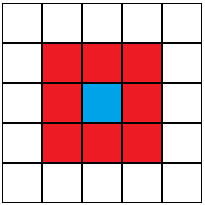
\includegraphics[width=.4\linewidth]{termitas/screen1.png}
    \captionof{figure}{Vecindad de Moore}
    \label{fig:vecindadmoore}
  \end{minipage}%
  \begin{minipage}{.5\textwidth}
    \centering
    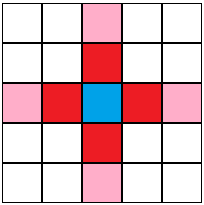
\includegraphics[width=.4\linewidth]{termitas/screen2.png}
    \captionof{figure}{Vecindad de Von Neumann de radio 1 (rojo) y radio 2 (rojo y rosa).}
    \label{fig:vecindadneumann}
  \end{minipage}
\end{figure}

Se tiene un estado inicial (al tiempo t=0) en el que se asigna un estado a cada célula. Una nueva generación es creada (avanzar t en 1) según alguna regla que determina el nuevo estado de cada célula en términos del estado actual de la célula y la de sus vecinos [Fig. ~\ref{fig:numtrans} ].\par

\begin{figure}
  \centering
  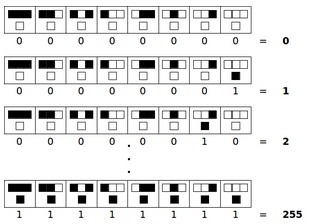
\includegraphics[width=0.6\textwidth]{termitas/screen3.png}
  \caption{Numeración de reglas de transición para autómatas celulares unidimensionales.}
  \label{fig:numtrans}
\end{figure}

\subsection{Modelo basado en agentes}
Un modelo basado en agentes es un tipo de modelo computacional que permite la simulación de acciones e interacciones entre individuos autónomos dentro de un entorno, y permite determinar qué efectos producen en el conjunto del sistema.\par

Combina elementos de teoría de juegos, sistemas complejos, emergencia, sociología computacional, sistemas multi-agente y programación evolutiva.
Los modelos simulan las operaciones simultáneas e interacciones de múltiples agentes, en un intento de recrear y predecir la apariencia de fenómenos complejos. El proceso de emergencia surge de un nivel bajo hacia niveles del sistema más altos. La clave es notar que reglas de comportamientos sencillos generan comportamientos complejos.\par

\subsection{Agentes aut\'onomos y auto-organizaci\'on}
Un agente autónomo es una unidad que interactúa con su entorno (el cual probablemente consta de otros agentes) pero actúa independientemente de todos los demás agentes porque no toma decisiones con respecto a algún líder o plan global a seguir. Es decir, cada agente actúa por sí mismo.\par

Así, veremos cómo múltiples agentes pueden desempeñar tareas que aparentan seguir un plan global. A este proceso en el que cada agente autónomo interactúa a su propia manera para crear un orden global se le conoce como auto-organización y se observa como modelos simples son capaces de generar comportamientos complejos.\par

\section{Planteamiento}

\subsection{Modelo de termitas}
Mitchel \cite{Resnick1994} estudió varios sistemas de agentes primitivos, uno de ellos fueron las termitas teóricas dentro de un espacio con astillas esparcidas que seguían las siguientes reglas:

\begin{itemize}
  \item Caminar aleatoriamente hasta encontrar una astilla.
  \item Si la termita está cargando una astilla, la suelta y continua caminando aleatoriamente.
  \item Si la termina no está cargando una astilla, la toma y continua caminando aleatoriamente con la astilla.
\end{itemize}

Claramente, las reglas definidas por Resnick son tan simples como es posible. No parece haber lugar para un comportamiento inteligente en un modelo como éste, tampoco parece que las termitas puedan producir nada con algún sentido más allá de la aleatoriedad de las astillas distribuidas en el entorno.\par

La Figura ~\ref{fig:termitasaleatorias} muestra seis escenarios de la simulación del conjunto de reglas simples con un conjunto pequeño de termitas. En la configuración inicial el universo de termitas consiste en una cuadrícula con astillas aleatoriamente distribuidas. La representación de la cuadrícula consta de una frontera periódica, es decir, un punto en una de las aristas de la cuadrícula tiene como vecinos a los puntos en la arista opuesta.
Al comenzar la simulación, las termitas mueven las astillas en pequeños grupos o clusters. Conforme pasa el tiempo, los clusters se vuelven más grandes y más definidos.\par

Tras cientos de miles de pasos en la ejecución de la simulación, como se muestra en la última imagen de la Figura 4, las astillas están claramente bien definidas en una colección. Obviamente esto es un método poco óptimo para coleccionar astillas, sin mencionar lo frustrante que es observar el proceso. Sin embargo, con el paso del tiempo es un hecho que el orden del sistema es evidente como resultado.\par

\begin{figure}
  \centering
  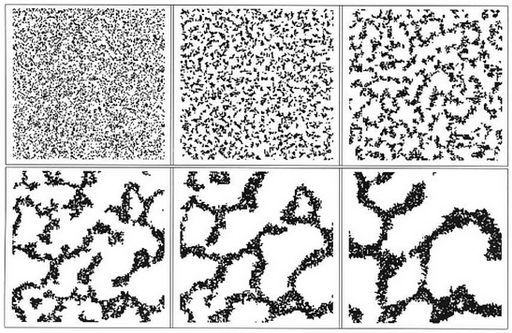
\includegraphics[width=0.9\textwidth]{termitas/screen4.png}
  \caption{Termitas colocando aleatoriamente astillas con las reglas definidas anteriormente.}
  \label{fig:termitasaleatorias}
\end{figure}

\section{Desarrollo e implementaci\'on}
Los resultados anteriores son reportados por el propio Resnick, sin embargo, para mostrar que es posible llegar al mismo resultado se lleva a cabo una implementación con el lenguaje de programación \classname{Processing}.
Al alumno se le proporciona parte de la implementación, de manera que se enfoque únicamente en programar el comportamiento descrito y evitando perder tiempo en la interfaz gráfica.

Las clases, métodos y variables más relevantes son las siguientes:
\pagebreak

\begin{description}%[leftmargin=40pt, labelindent=20pt]
  \item[Clase Celda] \hfill \\
    Representación de cada espacio dentro de la cuadrícula donde estarán las termitas y astillas.
    Cada celda tiene coordenadas (x,y) y un valor booleano para indicar si hay una astilla.

  \item[Clase Termita] \hfill \\
    Representación de una termita. Se representan las coordenadas (x,y) de su posición, la dirección en la que está observando (auxiliar que más adelante será mencionado a detalle) y un valor booleano para indicar si está cargando una astilla.

  \item[Clase ModeloTermitas] \hfill \\
    Representación de una colonia de termitas. Principalmente contiene una matriz de celdas (la representación del mundo) y una lista de termitas (nuestros agentes). Adicionalmente se define la cantidad de celdas a lo ancho y alto, un valor auxiliar para conocer la cantidad de iteraciones, un objeto de la clase Random (para hacer decisiones aleatorias) y el tamaño en pixeles de cada celda (para la visualización con Processing).
\end{description}

\subsection{Implementaci\'on}
El constructor de la clase \classname{ModeloTermitas} ya está implementado (principalmente para inicializar el espacio y termitas). También se encuentra implementado el método \classname{moverTermita}, que mueve la termita dada como parámetro en la dirección indicada. Cada termita tiene una vecindad de Moore, es decir, tienen 8 celdas adyacentes (considerando un espacio periódico) que se enumeran según la Fig. ~\ref{fig:dirsposibles1} \par

\begin{figure}
  \begin{center}
    \begin{tabular}{| l | c | r |}
      \hline
      0 & 1 & 2 \\ \hline
      7 &   & 3 \\ \hline
      6 & 5 & 4 \\
      \hline
    \end{tabular}
  \end{center}
  \caption{Las 8 posibles direcciones y vecindades de cada termita o celda.}
  \label{fig:dirsposibles1}
\end{figure}

De la misma manera se indica la dirección en la que puede mirar una termita. Por ejemplo, si la termita está mirando en dirección con valor 1 significa que está observando hacia arriba. Si tuviera el valor 4 significa que está observando en diagonal inferior derecha.

Existen 3 maneras diferentes de simular e implementar el modelo de termitas:

\begin{enumerate}
  \item \textbf{Usando las 8 posibles direcciones} \\
    Siguiendo la idea original con caminatas aleatorias en las 8 posibles direcciones para las termitas.


  \item \textbf{Modificar la caminata para que sea aleatoria y restringida} \\
    Una manera de avanzar totalmente aleatoria como en el primer caso implica que pueden existir muchos movimientos innecesarios (considerese la situación en la que una termita se cicla moviéndose en la casilla delante de ella y detrás de ella).
    Empleando la dirección en la que está observando la termita se puede restringuir su movimiento a solo 3 opciones: a la izquierda, al frente o a la derecha.
    Adicionalmente al soltar una astilla, la termita da media vuelta y se coloca en la dirección opuesta de donde soltó la astilla (esto evita una situación similar en la que se cicle una termita moviendo la misma astilla al mismo lugar).

  \item \textbf{Brindar un salto a las termitas} \\
    Esto significa que en el momento en que una termita suelta una astilla, en lugar de moverse en la dirección opuesta, las termitas “brincan” o se mueven a una celda sin astilla y continúan caminando de manera aleatoria y restringida.
\end{enumerate}

Cada una de las diferentes maneras de implementación se encuentran asignadas a los métodos \classname{evolucion1}, \classname{evolucion2} y \classname{evolucion3}, respectivamente.

El archivo \classname{Termitas.pde} contiene parte del código de la simulación y solamente tiene implementado la visualización de las termitas como cuadrados verdes moviéndose aleatoriamente (Fig. ~\ref{fig:sinastillas} ). Al implementar todos los métodos faltantes se darán cuenta de que cuando una termita está cargando una astilla (cuadros amarillos) cambia de color a rojo.


% Fig. 6. Captura de pantalla del código Termitas.pde de Processing
\begin{figure}
  \centering
  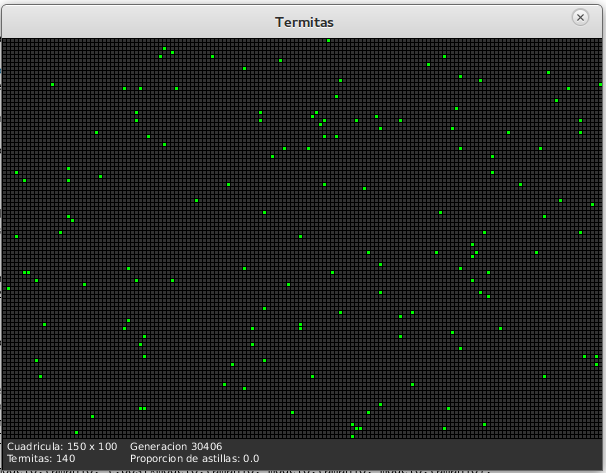
\includegraphics[width=0.7\textwidth]{termitas/sinastillas.png}
  \caption{Captura de pantalla del código \classname{Termitas.pde} de Processing.}
  \label{fig:sinastillas}
\end{figure}

Se debe implementar el comportamiento de las termitas para simular todo el sistema de la mejor manera. Dado que la interfaz gráfica está dada, solamente es necesario implementar los siguientes métodos:

\begin{itemize}
  \item \classname{int direccionAleatoriaFrente(int direccion)}
  \item \classname{boolean hayAstilla(Termita t, int direccion)}
  \item \classname{void dejarAstilla(Termita t, int direccion)}
  \item \classname{void dejarAstilla(Termita t)}
  \item \classname{void dejarAstillaConSalto(Termita t)}
  \item \classname{void tomarAstilla(Termita t, int direccion)}
\end{itemize}

Cada método se encuentra especificado dentro del archivo \classname{Termitas.java}.


\section{Requisitos y resultados}

Para evaluar y calificar la práctica es necesario que se implementen todos los métodos mencionados e indicados en el código, respetando implementar sólo lo que se pide (para evitar comportamientos extraños de la simulación).
Es completamente válido utilizar bibliotecas adicionales si lo consideran necesario, así como la creación y uso de sus propios métodos auxiliares si lo desean.

Debe notarse una mejora significativa mediante la implementación de la caminata restringida o el uso del salto. Es decir, verifiquen que tras varias iteraciones su implementación del modelo actúe como se espera. Las siguientes imágenes ilustran parte de los resultados esperados [Fig. ~\ref{fig:evo1} ] [Fig. ~\ref{fig:evo2} ] [Fig. ~\ref{fig:evo3} ].

\begin{figure}
  \centering
  \includegraphics[width=0.65\textwidth]{termitas/evo1.png}
  \caption{Simulación con idea original después de 10000 iteraciones (evolucion1).}
  \label{fig:evo1}
\end{figure}

\begin{figure}
  \centering
  \includegraphics[width=0.65\textwidth]{termitas/evo2.png}
  \caption{Empleando caminata aleatoria restringida tras 5000 iteraciones. La cantidad de astillas es la misma pero se observa un mejor ordenamiento y en menor tiempo.}
  \label{fig:evo2}
\end{figure}

\begin{figure}
  \centering
  \includegraphics[width=0.65\textwidth]{termitas/evo3.png}
  \caption{El uso de termitas con salto brinda una aproximación similar a la anterior. Cambiando algunos parámetros se pueden obtener resultados similares a colonias de termitas de la naturaleza.}
  \label{fig:evo3}
\end{figure}

% \subsection{Agradecimientos}
% \noindent Esta práctica fué realizada originalmente por Rodrigo Eduardo Colín Rivera (animeroy@gmail.com), las modificaciones hechas fueron mínimas, por lo que todo el crédito va para el. \\\\


% \begin{figure}[h]
%   \centering
%   \includegraphics[width=0.65\textwidth]{evo1.png}
%   \caption{Simulación con idea original después de 10000 iteraciones (evolucion1).}
%   \label{fig:evo1}
% \end{figure}

% \begin{figure}[h]
%   \centering
%   \includegraphics[width=0.65\textwidth]{evo2.png}
%   \caption{Empleando caminata aleatoria restringida tras 5000 iteraciones. La cantidad de astillas es la misma pero se observa un mejor ordenamiento y en menor tiempo.}
%   \label{fig:evo2}
% \end{figure}

% \begin{figure}[h]
%   \centering
%   \includegraphics[width=0.65\textwidth]{evo3.png}
%   \caption{El uso de termitas con salto brinda una aproximación similar a la anterior. Cambiando algunos parámetros se pueden obtener resultados similares a colonias de termitas de la naturaleza.}
%   \label{fig:evo3}
% \end{figure}





\chapter{Estados y espacio de búsqueda}
\chapterauthor{ %
  Rodrigo Eduardo Colín Rivera \\
  Verónica Esther Arriola Ríos
}



\section{Objetivo}
Que el alumno comprenda la noción de Estado y Espacio de Búsqueda, y que pueda representar en una estructura de datos todos los posibles estados de un mundo dado. \par

\section{Introducci\'on}
Dado un problema o modelo es posible determinar las características del mundo descrito en él. Uno de los puntos a tratar es la representación de dicho mundo y el concepto de estado. Un estado es una configuración posible del mundo con el que se trabaja. Por ejemplo, un juego de ajedrez se compone de un tablero de 64 cuadros donde inicialmente están 32 piezas (16 para cada jugador); El estado inicial del ajedrez se muestra en la Figura ~\ref{fig:ajedrez}.\par

\begin{figure}
  \centering
  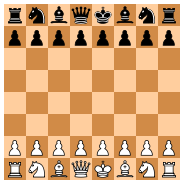
\includegraphics[width=0.4\textwidth]{estados/screen1.png}
  \caption{Estado inicial del juego de ajedrez.}
  \label{fig:ajedrez}
\end{figure}

Cuando una pieza se mueve, el estado del ajedrez cambia; pues la posición y cantidad de las piezas en juego determinan el estado del ajedrez.\par

\noindent De esta manera el espacio de estados se representa como una gráfica donde cada nodo representa un estado del problema y las aristas que los unen son la aplicación de un operador o función.\par


\begin{figure}
  \centering
  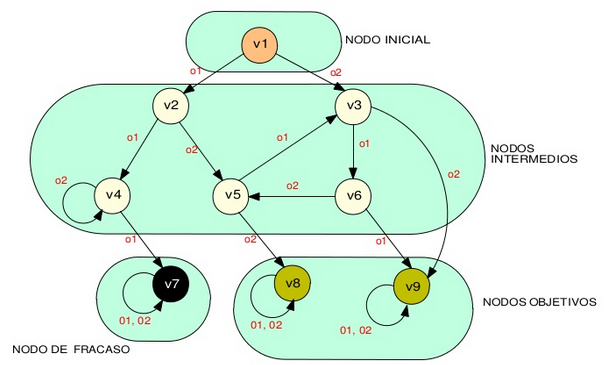
\includegraphics[width=0.9\textwidth]{estados/screen4.png}
  \caption{Ejemplo de un espacio de estados. \protect\footnotemark }
  \label{fig:espacioestados}
\end{figure}

\footnotetext{Milton A. Ram\i'rez Klapp, Notas de Inteligencia Artificial, Universidad San Sebasti\a'n, Facultad de Ingenier\i'a y Tecnolog\i'a.}

Es decir, el espacio de estados son todas las posibles configuraciones del problema. En el caso del ajedrez, las operaciones que unen cada estado en la gráfica representan el movimiento de una pieza por parte del jugador.\par


\section{Desarrollo e implementaci\'on}

La práctica consiste de generar los sucesores de los estados válidos del juego del Gato (también llamado Tres en línea).\par
Recordemos que el juego del Gato es entre dos jugadores, representados por los símbolos \enquote{\classname{X}} y \enquote{\classname{O}} que toman turnos para marcar los espacios de un tablero de 3x3.
Un jugador gana cuando logra tener una línea, ya sea horizontal, vertical o diagonal, de 3 símbolos correspondientes.\par

\begin{figure}
  \centering
  
\includegraphics[width=0.7\textwidth]{estados/screen2.png}
  \caption{Ejemplo de un juego de Gato donde gana el jugador \enquote{\classname{X}}. \protect\footnotemark}
  \label{fig:tictactoe}
\end{figure}

\footnotetext{Autor: Gdr (http://en.wikipedia.org/wiki/User:Gdr)}

Afortunadamente el juego del Gato es lo bastante simple como para evitar ciclarse al generar el espacio de estados y eso es una característica importante que ayuda a la construcción del espacio de estados ya que  podemos hacer uso de un árbol (que es un tipo especial de gráfica) para almacenar los estados.\par


\begin{figure}
  \centering
  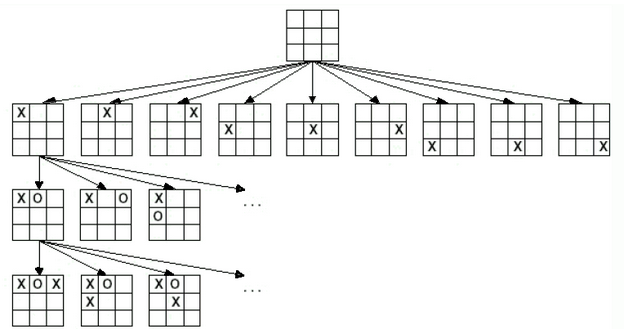
\includegraphics[width=0.8\textwidth]{estados/screen3.png}
  \caption{Espacio de estados del Gato representado como un árbol.}
  \label{fig:espaciogato}
\end{figure}

Por tanto, se necesitan los siguientes elementos para representar el espacio de estados del Gato:

\begin{enumerate}
  \item \textbf{Representación del estado} \hfill\par
    Una manera de representar el estado del Gato, se usará la siguiente idea:\medskip
    
    \classname{int[][] tablero = [[0,0,1], [0,0,0], [4,4,0]]}

    \begin{figure}[h!]
      \begin{center}
        \begin{tabular}{ l | l | l }
          % \hline
             &   & O \\ \hline
             &   &   \\ \hline
           X & X &   \\
          % \hline
        \end{tabular}
      \end{center}
      \caption{Representación gráfica del estado del Gato}
      \label{fig:representacionestado}
    \end{figure}

    Con \classname{1} representando al primer jugador y \classname{4} al segundo (fig~\ref{fig:representacionestado}).


  \item \textbf{Función generadora}\hfill \\
    Se necesitará implementar una función que genere los sucesores de un estado del juego del Gato, considerando sólo las jugadas válidas y descartando simetrías.

  \item \textbf{Función de comprobación} \hfill \\
    Ne necesitará implementar una función que verifique si hubo ganador en un estado dado, utilizando una bandera para indicar que no se debe generar sucesores de ese estado, para evitar generar estados inalcanzables.
\end{enumerate}


\subsection{Implementaci\'on}
Se volverá a trabajar con \classname{Processing}.

Se debe programar lo referente a generación de sucesores de un estado, verificación de simetrías y agregar variables que lleven el conteo de empates y juegos ganados por cada jugador, esto se imprimirá junto con la información de nodos del nivel generado.

\noindent En pocas palabras es necesario implementar los siguientes métodos:

\begin{itemize}
  \item \classname{LinkedList<Gato> generaSucesores()}
  \item \classname{boolean esSimetricoDiagonalInvertida(Gato otro)}
  \item \classname{boolean esSimetricoDiagonal(Gato otro)}
  \item \classname{boolean esSimetricoVerticalmente(Gato otro)}
  \item \classname{boolean esSimetricoHorizontalmente(Gato otro)}
  \item \classname{boolean esSimetrico90(Gato otro)}
  \item \classname{boolean esSimetrico180(Gato otro)}
  \item \classname{boolean esSimetrico270(Gato otro)}
\end{itemize}

\noindent Cada método se encuentra especificado dentro del archivo \classname{Gatos.java}.


\subsection{Punto extra}
Si lo desean pueden extenderse e implementar una función hash para cada estado generado, e implementar una lista cerrada. De esta manera se evita expandir rutas que ya se habían expandido anteriormente.Podrán obtener hasta \textbf{2} puntos extras.


\section{Requisitos y resultados}

Para evaluar y calificar la práctica es necesario que se implementen todos los métodos mencionados e indicados en el código, respetando implementar sólo lo que se pide (para evitar comportamientos extraños de la simulación).
Es completamente válido utilizar bibliotecas adicionales si lo consideran necesario, así como la creación y uso de sus propios métodos auxiliares si lo desean.

Deben correr su simulación de los espacios de estados del Gato sin simetrías, y después con ellas. Agreguen en su archivo \classname{readme} un pequeño párrafo detallando sus observaciones con respecto a lo anterior.

Si crean métodos auxiliares, no olviden documentar cual es su función.





\chapter[Retractación]{Recursión y Retractación (\textit{Backtrack})}
\chapterauthor{Rodrigo Eduardo Colín Rivera}



\section{Objetivo}
Comprender el algoritmo de búsqueda con retractación (\textit{backtrack}) y su relación con recursión. Llevar a cabo su implementación en la construcción de laberintos. Entender la forma de representar la lógica de la construcción del laberinto y su visualización. \par

\section{Introducci\'on}
\textbf{Retractación} es un algoritmo para encontrar soluciones en problemas computacionales donde se encuentran varios candidatos parciales de solución que se van descartando conforme avanza el algoritmo o la búsqueda.

El problema más clásico de la aplicación de retractación es el problema de las \textbf{ocho reinas}, que consiste en colocar ocho reinas en un tablero de ajedrez convencional de manera que ninguna ataque a las demás. En cada paso del algoritmo se agrega una reina a una casilla y se verifica que no ataque a las \textbf{k} reinas del tablero. Cuando no se cumple esta condición, se vuelve a una solución válida previa y se continúa probando hasta que satisfaga que no se ataquen ninguna de las reinas del tablero.\par

La aplicación de la técnica de retractación sólo tiene sentido en problemas que involucran soluciones parciales. Hay que notar que es una manera más eficiente que el uso de fuerza bruta, ya que se descartan muchas posibilidades que no cumplen los requisitos para ser solución del problema.

Conceptualmente, retractación es similar a la búsqueda en profundidad en árboles. Considerando que cada nodo en el árbol de búsqueda es una posible solución parcial del problema, la forma de recorrerlo es mediante recursión; podando o descartando subárboles que no son válidos como solución.\par


\section{Desarrollo e implementaci\'on}

\noindent Se desarrollará una aplicación que genera laberintos usando una interfaz gráfica.

\subsection{Algoritmo de construcci\'on del laberinto}

El objetivo de este algoritmo es construir un escenario que consiste en una serie de pasillos que cumplan con los requisitos siguientes:
\begin{itemize}
 \item Es posible llegar a cualquier punto del laberinto desde cualquier otro punto.  Es decir, no hay regiones cerradas inaccesibles.
 \item La ruta entre dos puntos cualquiera del laberinto es única.
\end{itemize}
Por lo tanto, es posible seleccionar un punto como \textit{inicio} y cualquie otro como \textit{destino} y existe un único camino entre ellos.

Para definir este problema se empleó el ejemplo de la siguiente página para ver la construcción (primer ejemplo: ``\textit{recursive backtracker}''):
\href{http://weblog.jamisbuck.org/2011/2/7/maze-generation-algorithm-recap}{Recursive Backtracker}
\footnote{http://weblog.jamisbuck.org/2011/2/7/maze-generation-algorithm-recap}
También hay una liga sobre el algoritmo y una implementación hecha en lenguaje Ruby:
\href{http://weblog.jamisbuck.org/2010/12/27/maze-generation-recursive-backtracking}{Maze generation}
\footnote{http://weblog.jamisbuck.org/2010/12/27/maze-generation-recursive-backtracking}

\noindent A continuación se explica la construcción del laberinto, con un algoritmo que satisface los requisitos anteriores:

\begin{enumerate}
  \item El algoritmo comienza con un tablero de celdas de tamaño N x M.
    \begin{figure}[h!]
      \centering
      
\includegraphics[width=0.2\textwidth]{retractacion/screen1.png}
      \caption{Ejemplo con N=6 y M=6.}
      \label{fig:tablero1}
    \end{figure}
    
  \item Se elige una celda aleatoriamente como la celda \textit{inicial}/actual, se marca como visitada y se agrega al stack.
    \begin{figure}[h!]
      \centering
      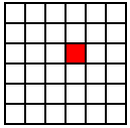
\includegraphics[width=0.2\textwidth]{retractacion/screen2.png}
      \caption{}
      \label{fig:tablero2}
    \end{figure}
    
  \item Se elige de manera aleatoria una dirección hacia donde moverse, esto consiste en elegir una casilla adyacente que no haya sido visitada. Dependiendo de la dirección elegida se debe borrar la pared correspondiente. Se marca como visitada la celda, se empuja a una pila de celdas y se actualiza la celda actual.
    \pagebreak
    \begin{figure}[h!]
      \centering
      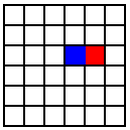
\includegraphics[width=0.2\textwidth]{retractacion/screen3.png}
      \caption{Ejemplo donde se elige la celda de la derecha. Se borra la pared entre las celdas y se marca la nueva celda actual (color rojo).}
      \label{fig:tablero3}
    \end{figure}
    
  \item El paso anterior se repite hasta que ya no haya direcciones por elegir, es decir, se queda encerrada la celda actual.
    \begin{figure}[h!]
      \centering
      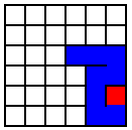
\includegraphics[width=0.2\textwidth]{retractacion/screen4.png}
      \caption{Tras algunos movimientos, la celda actual ya no puede seguir moviéndose.}
      \label{fig:tablero4}
    \end{figure}
    
  \item Estando encerrados sin poder elegir una celda adyacente sin visitar, se procede a explusar una celda de la pila para cambiar la posición de la celda actual y repetir el algoritmo desde el paso 3 hasta recorrer todo el tablero de celdas.
    \begin{figure}[h!]
      \centering
      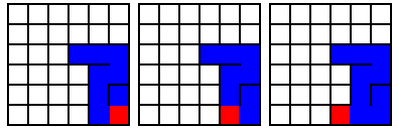
\includegraphics[width=0.6\textwidth]{retractacion/screen5.png}
      \caption{Ejemplo de un retroceso usando la pila y cambiando la celda actual.}
      \label{fig:tablero5}
    \end{figure}
    \pagebreak
    \begin{figure}[h!]
      \centering
      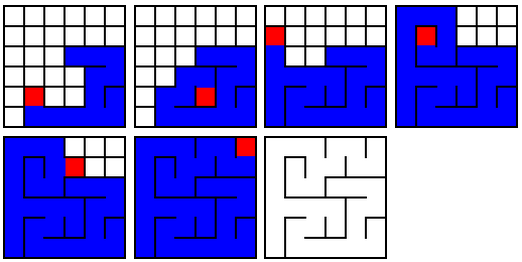
\includegraphics[width=0.6\textwidth]{retractacion/screen6.png}
      \caption{Ejemplo tras varios pasos del algoritmo hasta cubrir todo el tablero.}
      \label{fig:tablero6}
    \end{figure}
\end{enumerate}


\subsection{Implementaci\'on}

Se debe implementar tanto la lógica de construcción del laberinto como su visualización. Se recomienda usar \classname{Processing/Java} ya que solo requiere usar las primitivas de dibujo: \classname{stroke()} y \classname{line()}. Adicionalmente también pueden usar: \classname{fill()} y \classname{rect()}. Es recomendable usar los siguientes métodos para una adecuada visualización: \classname{background()} y \classname{size()}.



\section{Requisitos y resultados}

Para llevar a cabo la evaluación de esta práctica es necesario implementar la construcción del laberinto usando retractación. Empleen como estructura auxiliar durante la construcción una pila o stack.

La implementación debe ser lo más generalizada y robusta posible, es decir, se deben definir parámetros o valores para determinar el ancho y largo del laberinto.

No olviden documentar su código. De preferencia utilicen el estándar de \classname{JavaDoc}, de no hacerlo, al menos describan de manera breve, clara y concisa el funcionamiento de sus métodos. Si omiten documentación en su código les afectará negativamente en su calificación.

El ejemplo visto en laboratorio se construye en tiempo de ejecución. Es deseable que se muestre esta construcción pero no es necesaria. Es válido mostrar el resultado final aunque no se visualice la construcción.

Si todo se implementa correctamente debe ser posible generar diferentes tamaños de laberintos.



% \subsection{Agradecimientos}
% \noindent Esta práctica fue realizada originalmente por Rodrigo Eduardo Colín Rivera (animeroy@gmail.com). Se hicieron algunas modificaciones, pero sigue mereciendo crédito por su labor. \\\\





\chapter{Recocido simulado}
\chapterauthor{ %
  Benjamín Torres Saavedra \\
  Verónica Esther Arriola Ríos
}


\section{Objetivo}

Que el alumno se familiarice con una estrategia de mejoramiento iterativa para la resolución de problemas conocida como recocido simulado.



\section{Introducción}

\subsection{Recocido simulado}

Este algoritmo puede ser visto como una mejora al algoritmo de ascenso de colinas, el cual mejora de manera iterativa una representación de la solución a un problema hasta que se encuentre el óptimo o se estanque en un máximo local.  Recocido simulado integra una selección de soluciones estocástica, es decir, para elegir la siguiente solución no siempre se escoge la mejor, con la cual se le da la libertad de explorar zonas distintas del espacio de soluciones, en las cuales el ascenso de colinas puede detenerse fácilmente.

El pseudocódigo de este algoritmo es descrito en el \cite{Russell2010} en la sección de algoritmos de mejoramiento iterativo y lo podemos ver en el \pref{alg:annealing}.

\begin{algorithm}
 \caption{Recocido simulado}\label{alg:annealing}
 \begin{algorithmic}
  \Function{RecocidoSimulado}{$problema$, $horario$}
    \State \# $problema$: un problema
    \State \# $horario$: mapeo de $tiempo$ a $temperatura$.
    \State $actual \leftarrow $ \Call{HazNodo}{EstadoInicial(problema)}
    \For{$t \leftarrow 1$ a $\infty$}
      \State $T \leftarrow horario(t)$
      \If {$T < \varepsilon$} \Return $actual$ \EndIf
      \State $siguiente \leftarrow$ un sucesor de $actual$ elegido al azar.
      \State $\Delta E \leftarrow$ \Call{Valor}{$siguiente$} - \Call{Valor}{$actual$}
      \If {$\Delta E > 0$}
        \State $actual \leftarrow siguiente$
      \Else
        \State $actual \leftarrow siguiente$ sólo con probabilidad $e^{\frac{\Delta E}{T}}$
      \EndIf
    \EndFor
  \EndFunction
 \end{algorithmic}
\end{algorithm}



\subsection{Problema del agente viajero (TSP)}

Este problema consiste en encontrar, dada una lista de ciudades, una ruta que pueda seguir un agente para recorrer todas las ciudades y volver a aquella en la cual inició el viaje.  Para que este recorrido valga la pena debe ser lo más económico posible o, en su defecto, recorrer la menor distancia que permita visitar todas las ciudades.

Este problema es ampliamente conocido por ser de la clase NP-Completo, es decir, que no se puede resolver en tiempo polinomial por algoritmos deterministas, afortunadamente para esta práctica no usaremos un algoritmo de tal tipo y podremos aproximarnos a una solución en un tiempo razonable.



\section{Desarrollo e implementaci\'on}

Se les proporcionará código fuente en Java, que deberán completar con la finalidad de resolver el problema del agente viajero.

El código fuente se encuentra en los archivos \code{Solucion.java}, es que se encargará de representar a una ruta del agente viajero que pase por todas las ciudades y el archivo \code{RecocidoSimulado.java}, que implementará el algoritmo anteriormente descrito.

\subsection{Implementaci\'on}

Se debe programar una clase hija de \code{Solución}.  Esta clase hija agregará los atributos del(de los) tipo(s) necesario(s) para representar una propuesta de solución al problema que se desea resolver.

En la página \hurl{http://www.math.uwaterloo.ca/tsp/world/countries.html\#DJ} se pueden encontrar una serie de países con ciudades y sus correspondientes coordenadas.  Sin asumes una conectividad total de las ciudades y usas la distancia euclideana como métrica, tu tarea será tratar de aproximarte lo mejor posible a la longitud del camino óptimo de la ciudad seleccionada.  Puedes incorporar la información a tu programa como te sea más conveniente.

Los métodos a implementar dentro de una clase hija de \code{Solución} son:
\begin{itemize}
 \item Un constructor.
 
 Este método deberá inicializar una representación con una propuesta para solución de un problema, en nuestro caso, una ruta del problema del agente viajero.  Deberás elegir cómo representar la solución.  No es necesario que dicha solución sea correcta.
 
 En el caso del agente viajero puede ser que la solución visite todas las ciudades, pero que la distancia recorrida no sea mínima y/o que las visite más de una vez.
 
 \item \code{public Solución siguienteSolución()}
 
 Genera una nueva solución perturbando de manera aleatoria al objeto que lo llama.  Observa que al sobreescribir el método puedes cambiar el tipo de regreso para evitar hacer audiciones (\textit{castings}).
 
 \item \code{public float evaluar()}
 
 Califica la solución actual según la heurística elegida de acuerdo al problema a resolver.
\end{itemize}


Para la clase \code{RecocidoSimulado}:
\begin{itemize}
 \item \code{public RecocidoSimulado()}
 
 Inicializa los parámetros del algoritmo. En principio ya funciona así, pero la puedes modificar si lo consideras necesario.
 
 \item \code{public float nuevaTemperatura()}
 
 Calcula la nueva temperatura, se espera que a lo largo de las iteraciones este valor decrezca, llegando a cero en el último paso.
 
 \item \code{public Solucion seleccionarSiguienteSolución()}
 
 Dada la solución actual, este método debe modificarla para obtener una solución nueva y elegir esta nueva solución con cierta probabilidad dependiendo de si es mejor o no, según el algoritmo presentado anteriormente.
 
 \item \code{public Solución ejecutar()}
 
 Ejecuta el algoritmo con los parámetros inicializados, puedes modificar la firma si lo consideras necesario.
\end{itemize}

Finalmente, en la clase \code{Main} únicamente se crea un objeto tipo \code{RecocidoSimulado} que ejecuta el algoritmo por algún número de iteraciones:
\begin{itemize}
 \item Calcula los parámetros para el constructor de\code{RecocidoSimulado}:
 
 \begin{itemize}
  \item Crea un objeto de la clase hija de \code{Solucion} que implementaste.
  
  \item Calcula la temperatura inicial y decaimiento adecuados para ejecutar recocido simulado dependiendo del número de interacciones.
 \end{itemize}

 \item Modificar el ciclo para monitorear la evolución del algoritmo entre interacciones.
\end{itemize}


\subsection{Punto extra}

Realiza las modificaciones que consideres pertinentes para poder utilizar una estrategia similar al recocido simulado para minimimzar la siguiente función:
\begin{align*}
 f(x,y) &= -20 e^{-0.2 \sqrt{0.5(x^2 + y^2)}} - e^{0.5 (\cos(2 \pi x) + \cos(2 \pi y))} + e + 20
\end{align*}
para $-5 \leq x,y \leq 5$.


\section{Requisitos y resultados}

El código debe ser implementado de manera eficiente y estar documentado para esclarecer su funcionamiento.  Además, debe encontrar una solución válida al problema del agente viajero.




\chapter{A*}


\section{Objetivo}
Que el alumno implemente y refuerce su comprensión del algoritmo A* \par

\section{Introducci\'on}

Resolveremos el problema de navegación en videojuegos con mundos hechos de mosaicos, utilizando el algoritmo A*, siguiendo el ejemplo de Patrick \cite{Lester2003}.

Vamos a asumir que tenemos un personaje que quiere ir desde un punto A hasta un punto B, y que ambos puntos están separados por una pared. Este ejemplo se puede apreciar en la figura~\ref{fig:fig1P4}, donde el cuadrado verde es el punto A, el rojo es el punto B y el rectángulo azul la pared mencionada anteriormente.

\begin{figure}
  \centering
  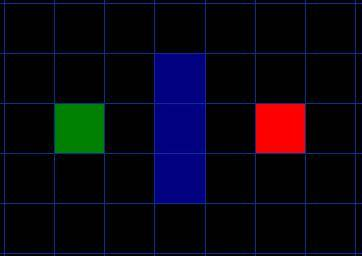
\includegraphics[width=0.4\textwidth]{aestrella/screen1.jpg}
  \caption{Escenario construido con mosaicos discretos. El problema de búsqueda de caminos consiste en encontrar una ruta desde el cuadro verde al cuadro rojo.}
  \label{fig:fig1P4}
\end{figure}

El primer paso que debemos hacer es simplificar el área de búsqueda, dividiendo nuestro mundo en una rejilla cuadrada. Con esto, podremos representar el mundo con una matriz bidimensional. Cada posición en la matriz representará un mosaico del mundo, el cual será transitable o no transitable. Entonces, el objetivo del algoritmo A* es calcular a que mosaico nos debemos mover en cada turno para lograr llegar al punto B. Una vez calculado esto, el personaje del juego se moverá del centro del mosaico donde se ecnuentra actualmente al centro del mosaico obtenido con A*.

A los puntos centrales dentro del mosaico se les llama \classname{nodos}. Esto ya que pudimos haber dividido el mundo en círculos, o en tríangulos. Cada mundo tendrá características diferentes, y se podrá simplificar de distintas formas.

\subsection{Iniciando la b\'usqueda}

Después de haber simplificado el área de búsqueda en nodos, el siguiente paso es dirigir una búsqueda para encontrar el camino más corto. En el algoritmo A*, lo hacemos empezando desde el punto A, comprobando los cuadros adyacentes (estados sucesores) y generalmente buscando hacia fuera hasta que encontremos nuestro destino.

\noindent Empezamos la búsqueda haciendo lo siguiente:

\begin{enumerate}
  \item Empezamos en el punto inicial A y lo añadimos a una \textbf{lista abierta} de cuadrados a tener en cuenta. La lista contiene los cuadrados que podrían formar parte del camino que queremos tomar, pero que quizás no lo hagan. Básicamente, esta es una lista de los cuadrados que necesitan ser considerados.
  \item Nos fijamos en todos los cuadrados alcanzables o transitables adyacentes al punto de inicio, ignorando cuadrados con muros, agua u otros terrenos prohibidos. Se añaden a la lista abierta también. Por cada uno de esos cuadrados, guardamos el punto A como su \textbf{cuadrado padre}. El cuadrado padre es muy importante para trazar nuestro camino.
  \item Sacamos el cuadro inicial A desde la lista abierta y lo añadimos a una \textbf{lista cerrada} de cuadrados que no necesitan ser vistos de nuevo.
\end{enumerate}

En este punto, se tendrá algo como la figura~\ref{fig:fig2P4}. En este diagrama, el cuadrado verde oscuro del centro es el cuadrado de inicio. Está bordeado de azul claro para indicar que el cuadrado ha sido añadido a la lista cerrada. Todos los cuadros adyacentes están ahora en la lista abierta para ser considerados. Cada uno tiene un puntero gris que señala a su padre, el cual es el cuadro inicial.

\begin{figure}[h]
  \centering
  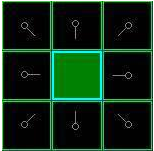
\includegraphics[width=0.3\textwidth]{aestrella/screen2.png}
  \caption{Mosaicos en la lista abierta con referencia a su padre.}
  \label{fig:fig2P4}
\end{figure}


Después, elegimos uno de los cuadrados adyacentes de la lista abierta y más o menos repetimos el proceso anterior. Pero, ¿qué cuadro se debe elegir? Aquel que tenga costo estimado \(f(n)\) más bajo.

\subsection{Puntuando el camino}

La clave para determinar qué cuadrados usaremos para resolver el camino está en la siguiente ecuación:\medskip

\begin{center}
\(f(n) = g(n) + h(n)\)
\end{center}\medskip

donde:

\begin{itemize}
  \item \(g(n)\) es el costo del movimiento para ir desde el punto inicial A a un cierto cuadro de la rejilla (\(n\)), siguiendo el camino generado para llegar ahí.
  \item \(h(n)\) es el costo del movimiento estimado para ir desde ese cuadro de la rejilla (\(n\)) hasta el destino final, el punto B. Esto se conoce como la heurística. Aquí se verá una forma de calcular la heurística, pero no es la única.
\end{itemize}

Nuestro camino se genera al ir repetidamente a través de nuestra lista abierta y eligiendo el cuadrado con la puntuación \(f(n)\) más baja. Este proceso se describirá con más detalle un poco más adelante. Primero veamos más de cerca cómo calculamos esta puntuación.

Tal y como está descrito arriba, \(g(n)\) es el costo del movimiento para ir desde el punto de inicio a un cuadro \(n\) usando el camino generado para llegar ahí. En esta práctica asignaremos un costo de 10 a cada cuadro vertical u horizontal hacia el que nos movamos, y un costo de 14 para un movimiento diagonal. Usamos estos números ya que es más simple poner 14 que \(\sqrt{2}^2\times10\) y porque usar números enteros es mucho más rápido para la computadora. Pronto descubrirás que los algoritmos de búsqueda pueden ser muy lentos si no usas atajos como este.

Ahora que hemos calculado el costo \(g(n)\) mediante un camino específico hasta cierto cuadro, la forma de resolver el costo \(g(n)\) del cuadro es tomar el costo \(g(n)\) de su padre, y luego añadirle 10 o 14 dependiendo de si está en diagonal u ortogonal con respecto al cuadro padre.

\(h(n)\) puede ser estimado de diferentes maneras. El método que usaremos aquí se llama el método Manhattan, donde se calcula el número total de cuadros movidos horizontalmente y verticalmente para alcanzar el cuadrado destino desde el cuadro actual, sin hacer uso de movimientos diagonales e ignorando cualquier obstáculo. Luego multiplicamos el total por 10. Se llama método Manhattan porque es como calcular el número de manzanas que hay desde un lugar a otro, donde no puedes acortar atravesando en diagonal una manzana. Es una estimación de la distancia que queda, no de la distancia actual, es por eso que se llama heurística.

\(f(n)\) se calcula sumando \(g(n)\) y \(h(n)\). El resultado del primer paso en nuestra búsqueda puede verse en la figura~\ref{fig:fig3P4}. Las puntuaciones \(f(n)\), \(g(n)\) y \(h(n)\) están escritas en cada cuadrado. En el cuadro inmediatamente a la derecha del cuadro inicial, se escribieron las letras F, G y H para indicar dónde se encuentran los valores de \(f(n)\), \(g(n)\) y \(h(n)\).

\begin{figure}[h!]
  \centering
  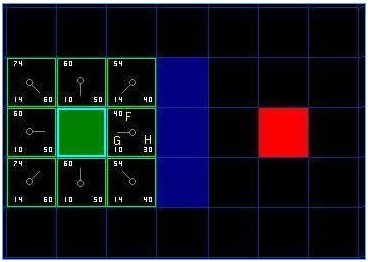
\includegraphics[width=0.5\textwidth]{aestrella/screen3.png}
  \caption{Cálculo de \(f\),\(g\) y \(h\) que se agregan a la lista abierta.}
  \label{fig:fig3P4}
\end{figure}

Así pues, obsevaremos algunos ejemplos de estos cuadros. En el cuadrado con letras, \(g(n)=10\). Esto es debido a que está solo a un cuadro del cuadrado inicial en dirección horizontal. Los cuadrados inmediatamente encima, abajo y a la izquierda del cuadrado inicial; tienen todos el mismo valor \(g(n)\) de 10. Los cuadros diagonales tienen un valor \(g(n)\) de 14.

Las puntuaciones \(h(n)\) se calculan estimando la distancia Manhattan hasta el cuadrado rojo objetivo, moviéndose solo horizontal y verticalmente e ignorando el muro que está en el camino. Usando este método, el cuadro a la derecha del inicial, está a 3 cuadros del cuadrado rojo con una puntuación \(h(n)\) de 30. El cuadrado está a sólo 4 cuadros de distancia (recuerda que solo nos movemos en dirección horizontal y vertical) con una puntuación \(h(n)\) de 40. Probablemente podrás calcular las puntuaciones \(h(n)\) para los demás cuadros.


\subsection{Continuando la b\'usqueda}

Para continuar la búsqueda, simplemente elegimos la puntuación \(f(n)\) más baja de todos aquellos que estén en la lista abierta. Para que esta operación se realize lo más eficientemente posible, la lista abierta se implementará con una cola de prioridades. Después hacemos lo siguiente con el cuadro seleccionado:

\begin{enumerate}
  \item Lo sacamos de la lista abierta y lo añadimos a la lista cerrada.  

  \item Comprobamos todos los cuadrados adyacentes, ignorando aquellos que estén en la lista cerrada o que sean intransitables: terrenos con muros, agua o cualquier terreno prohibido; añadimos los cuadros a la lista abierta si no están ya en esa lista. Hacemos que el cuadro seleccionado sea el \textbf{padre} de los cuadros nuevos.

  \item Si el cuadro adyacente ya está en la lista abierta, comprobamos si el camino nuevo a ese cuadro es mejor que el que tenía, es decir, si el valor de \(g(n)\) con este padre es menor que el que se había estimado con su padre anterior. Si no es así, no haremos nada. Por otro lado, si el costo \(g(n)\) del nuevo camino es más bajo, cambiamos el padre del cuadro adyacente al cuadro seleccionado (en el diagrama superior, cambia la dirección del puntero para que señale al cuadro seleccionado). Finalmente, recalculamos \(f(n)\) y \(g(n)\) de ese cuadrado.
\end{enumerate}


\section{Desarrollo e implementaci\'on}

La práctica consiste en implementar el algoritmo A* y generar una visualización de éste resolviendo un problema. Ustedes pueden modificar el mundo del problema, para que puedan ver cómo se comporta A* con distintas localizaciones de obstáculos y de nodos de inicio y fin. 


\subsection{Implementaci\'on}


Se debe programar lo referente al algoritmo A* y la función heurística.
También necesitarán implementar sus listas abierta y cerrada (o usar alguna biblioteca o clase ya implementada de \classname{Java}).
Se volverá a trabajar con \classname{Processing}.

\noindent Los métodos que deberán implementar son los siguientes:

\begin{enumerate}
  \item \classname{calculaHeuristica(Mosaico meta)}
  \item \classname{expandeNodoSiguiente()}
\end{enumerate}

\noindent Cada método se encuentra especificado dentro del archivo \classname{AEstrella.java}.


\section{Requisitos y resultados}

Para evaluar y calificar la práctica es necesario que se implementen todos los métodos mencionados e indicados en el código, respetando implementar sólo lo que se pide (para evitar comportamientos extraños de la simulación).
Es completamente válido utilizar bibliotecas adicionales si lo consideran necesario, así como la creación y uso de sus propios métodos auxiliares si lo desean.

Si crean métodos auxiliares, no olviden documentar cual es su función.


%  \begin{thebibliography}{1}

%   \bibitem{notes} Patrick Lester {\em A* Pathfinding para Principiantes}  2003 :
%   http://www.policyalmanac.org/games/articulo1.htm .

% \end{thebibliography}




\chapter{Factores}
\chapterauthor{%
  Luis Alfredo Lizárraga Santos \\
  Verónica Esther Arriola Ríos
}

\section{Objetivo}
Que el alumno implemente una clase \classname{Factor} para familiarizarse con las operaciones entre factores que se utilizan para realizar inferencia en redes Bayesianas

\section{Introducción}

\begin{definition}[Factor]
 \quotes{Sea \(D\) un conjunto de variables aleatorias [y $Val(D)$ una asignación de valores a estas variables]. Se define un Factor $\phi$ como una función de \(Val(D)\) a \(\mathbb{R}\). Un factor es no-negativo si todas sus entradas son no negativas. Al conjunto de variables \(D\) se le llama \textit{alcance del factor} y se denota como \(Alcance(\phi)\)}
 
 \parencite[104]{KollerFriedman2009}.
\end{definition}

Tomando como base la definición de Koller Y Friedman, podemos realizar un parafraseo y afirmar que un Factor es \quotes{Una estructura matemática definida sobre un conjunto de variables donde cada variable puede tomar valores de su dominio, el cual debe ser finito. A este conjunto de variables se les denomina como el alcance del factor; el factor asocia un número real a cada posible asignación de valores de esas variables}.

En cuanto a las operaciones de Factores que se explicarán en esta práctica, nos basamos en las operaciones que presentan Koller Y Friedman y que se utilizan en la materia: multiplicación, reducción, marginalización y normalización.

Utilizaremos a los factores para realizar operaciones con distribuciones de probabilidad, sin embargo es importante notar que, debido a la misma definición del Factor, el resultado de cada operación entre factores no siempre será una medida de probabilidad, pues esta limita su valores al intervalo $[0,1]$, mientras que los factores ocupan todo \(\mathbb{R}\).  Adicionalmente, sus operaciones no siempre incluyen las normalizaciones requeridas por las distribuciones de probabilidad; pero esto se convertirá en una ventaja para nosotros, como veremos más adelante.

\subsection[Operaciones]{Operaciones entre Factores}

\subsubsection{Multiplicación}

\begin{definition}[Multiplicación]
\quotes{Sean $X$, $Y$ y $Z$ tres conjuntos disjuntos de variables, y sean $\phi_1(X,Y)$ y $\phi_2(Y,Z)$ dos factores. Se define el Factor producto $\phi_1(X,Y) \times \phi_2(Y,Z)$ como un factor $\psi: Val(X,Y,Z) \mapsto \mathbb{R}$ de la siguiente forma: \[ \psi(X,Y,Z) = \phi_1(X,Y) \cdot \phi_2(Y,Z)\]}

\parencite[107]{KollerFriedman2009}.
\end{definition}

La operación de multiplicación es sencilla. Si los conjuntos de variables de los factores a multiplicar no tienen elementos en común, se multiplica cada entrada del factor A por cada entrada del Factor B. El alcance del factor resultante es la unión de los alcances de los factores a multiplicar \parencite[107]{KollerFriedman2009}.


\begin{figure}
    \centering
    \begin{subfigure}[b]{0.3\textwidth}
        \centering
        \begin{tabular}{ l | r }
          A & $\phi$(A)\\ \hline
          0 & .3  \\ \hline
          1 & .7  \\
        \end{tabular}
        \caption{Factor $A$}
    \end{subfigure}
    ~ 
    \begin{subfigure}[b]{0.3\textwidth}
        \centering
        \begin{tabular}{ l | r }
          B & $\phi$(B)\\ \hline
          0 & .6  \\ \hline
          1 & .4  \\
        \end{tabular}
        \caption{Factor $B$}
    \end{subfigure}
    ~
    \begin{subfigure}[b]{0.3\textwidth}
        \centering
        \begin{tabular}{ l | r }
          C & $\phi$(C)\\ \hline
          0 & .2  \\ \hline
          1 & .8  \\
        \end{tabular}
        \caption{Factor $C$}
    \end{subfigure}
    \caption{Factores sobre variables aleatorias binarias.}\label{fig:ABC}
\end{figure}

Por ejemplo: Tenemos los tres factores $A$, $B$ y $C$ de la \fref{fig:ABC}. Para obtener el factor $A \times B$, se multiplicaría el renglón $A=0$ con $B=0$, luego $A=0$ con $B=1$, $A=1$ con $B=0$ y por último $A=1$ con $B=1$ como en la \fref{fig:FactorAB}.

\begin{figure}[H]
  \begin{center}
    \begin{tabular}{ l  c | r }
      A & B & $\phi$(A,B)\\ \hline
      0 & 0 & (.3)*(.6) = 0.18 \\ \hline
      0 & 1 & (.3)*(.4) = 0.12 \\ \hline
      1 & 0 & (.7)*(.6) = 0.42 \\ \hline
      1 & 1 & (.7)*(.4) = 0.28 \\
    \end{tabular}
  \end{center}
  \caption{Factor $A \times B$}
  \label{fig:FactorAB}
\end{figure}

\noindent Si el alcance de ambos factores tiene variables en común, se debe asegurar que tengan el mismo valor en cada renglón por multiplicar en ambos factores. Por ejemplo, si se tienen los factores $A \times B$ y $A \times C$, al momento de multiplicar el renglón $\{A=0,B=0\}$ se debe seleccionar los renglones donde $A=0$ en el factor $A \times C$, estos son $\{A=0,C=0\}$ y $\{A=0,C=1\}$, como muestran \fref{fig:FAFB} y \fref{fig:FactorABC}.

\begin{figure}[h!]
    \centering
    \begin{subfigure}[b]{0.4\textwidth}
        \centering
        \begin{tabular}{ l  c | c }
          A & B & $\phi$(A,B)\\ \hline
          0 & 0 & (.3)*(.6) = 0.18 \\ \hline
          0 & 1 & (.3)*(.4) = 0.12 \\ \hline
          1 & 0 & (.7)*(.6) = 0.42 \\ \hline
          1 & 1 & (.7)*(.4) = 0.28 \\
        \end{tabular}
        \caption{Factor $A \times B$}
    \end{subfigure}
    ~ 
    \begin{subfigure}[b]{0.4\textwidth}
        \centering
        \begin{tabular}{ l  c | c }
          A & C & $\phi$(A,C)\\ \hline
          0 & 0 & (.3)*(.2) = 0.6 \\ \hline
          0 & 1 & (.3)*(.8) = 0.24 \\ \hline
          1 & 0 & (.7)*(.2) = 0.14 \\ \hline
          1 & 1 & (.7)*(.8) = 0.56 \\
        \end{tabular}
        \caption{Factor $A \times C$}
    \end{subfigure}
    \caption{Multiplicandos.}
    \label{fig:FAFB}
\end{figure}


\begin{figure}[H]
  \begin{center}
    \begin{tabular}{ l  l  c | c }
      A & B & C & $\phi$(A,B,C)\\ \hline
      0 & 0 & 0 & [(.3)*(.6)]*[(.3)*(.2)] = 0.0108  \\ \hline
      0 & 0 & 1 & [(.3)*(.6)]*[(.3)*(.8)] = 0.0432 \\ \hline
      0 & 1 & 0 & [(.3)*(.4)]*[(.3)*(.2)] = 0.0072 \\ \hline
      0 & 1 & 1 & [(.3)*(.4)]*[(.3)*(.8)] = 0.0288 \\ \hline
      1 & 0 & 0 & [(.7)*(.6)]*[(.7)*(.2)] = 0.0588 \\ \hline
      1 & 0 & 1 & [(.7)*(.6)]*[(.7)*(.8)] = 0.2352 \\ \hline
      1 & 1 & 0 & [(.7)*(.4)]*[(.7)*(.2)] = 0.0392 \\ \hline
      1 & 1 & 1 & [(.7)*(.4)]*[(.7)*(.8)] = 0.1568 \\ 
    \end{tabular}
  \end{center}
  \caption{Factor $(A \times B) \times (A \times C)$}
  \label{fig:FactorABC}
\end{figure}

Es importante hacer notar que al multiplicar los factores $A \times B$ y $A \times C$ no se estaría obteniendo la probabilidad conjunta de $A$, $B$ y $C$, si no alguna otra función $\phi(A,B,C)$. 

\subsubsection{Reducción}

\begin{definition}[Reducción]
\quotes{Sea $\phi(Y)$ un factor y \(U = u\) una asignación para \(U \subseteq Y\). Se define la reducción de un factor $\phi$ al contexto \(U = u\), denotado como \(\phi[U = u]\) (y abreviado como $\phi[u]$), como un factor con alcance \(Y' = Y - U\) de tal forma que \[\phi[u](y') = \phi(y',u)\]}

\parencite[111]{KollerFriedman2009}.
\end{definition}

La operación de reducción consiste en tomar un valor de alguna variable del factor y sólo tomar los renglones que cumplen con el valor dado de la variable. Por ejemplo: Se tiene el factor AB,

\begin{figure}[H]
  \begin{center}
    \begin{tabular}{ l  c | r }
      A & B & $\phi$(A,B)\\ \hline
      0 & 0 & .18  \\ \hline
      0 & 1 & .12  \\ \hline
      1 & 0 & .42  \\ \hline
      1 & 1 & .28  \\
    \end{tabular}
  \end{center}
  \caption{Factor AB}
  % \label{fig:FactorA}
\end{figure}

\noindent Si se desea reducir con A = 0, el resultado sería un factor:

\begin{figure}[h]
  \begin{center}
    \begin{tabular}{ l | r }
      B & \(\phi(B)\)\\ \hline
      0 & .18  \\ \hline
      1 & .12  \\
    \end{tabular}
  \end{center}
  \caption{Factor \(B\)}
  % \label{fig:FactorA}
\end{figure}

\subsubsection{Normalización}
Para normalizar un factor, esto es, que los valores que toma el factor sumen 1, basta con sumar todos los valores asociados a las asignaciones y dividir cada uno entre esta suma. Por ejemplo: Tenemos el factor \(\phi(B)\), la suma de sus posibles valores es .3, entonces tendríamos:

% TODO: Cambiar por un factor de probabilidad conjunta, donde no sumen uno sus renglones
\begin{figure}[H]
  \begin{center}
    \begin{tabular}{ l  c | r }
      A & B &  \(\phi(B)\)\\ \hline
      0 & 0 & (.18/.3)= .6  \\ \hline
      0 & 1 & (.12/.3)= .4 \\
    \end{tabular}
  \end{center}
  \caption{Factor \(B\)}
  % \label{fig:FactorA}
\end{figure}

% \noindent Esta operación es útil cuando se desea calcular probabilidades condicionales.

\subsubsection{Marginalización}
\quotes{Sea $X$ un conjunto de variables y sea \(Y \notin X\) una variable y $\phi(X,Y)$ un factor. Se define la marginalización de $Y$ en $\phi$, denotado como \(\sum_Y \phi\), como un factor $\psi$ sobre $X$ de tal forma que \[\psi(X) = \sum_Y \phi(X,Y)\]} \parencite[297]{KollerFriedman2009}.

La operación de marginalización consiste en tomar la variable a marginalizar, sumar los valores en los renglones en que cambia su valor pero el de las demás variables no, y asignar esta suma al renglón correspondiente de las variables restantes. Por ejemplo: tenemos el factor AB y deseamos marginalizar la variable B. Entonces, tomamos los renglones donde A=0 y los sumamos, tomamos los renglones donde A=1 y los sumamos:

\begin{figure}[H]
    \centering
    \begin{subfigure}[b]{0.4\textwidth}
        \centering
        \begin{tabular}{ l l  c | r }
           & A & B & $\phi$(A,B)\\ \cline{2-4}
          \(\to\) & 0 & 0 & .18  \\ \cline{2-4}
          \(\to\) & 0 & 1 & .12  \\ \cline{2-4}
           & 1 & 0 & .42  \\ \cline{2-4}
           & 1 & 1 & .28  \\
        \end{tabular}
        \caption{Factor AB}
    \end{subfigure}
    ~ 
    \begin{subfigure}[b]{0.4\textwidth}
        \centering
        \begin{tabular}{l  l | r }
            & A & $\phi$(A)\\ \cline{2-3}
        \(\to\) & 0 & (.18)+(.12)  \\
        \end{tabular}
        \caption{Factor A}
    \end{subfigure}
    \caption{Paso 1}
\end{figure}

% \noindent y

\begin{figure}[H]
    \centering
    \begin{subfigure}[b]{0.4\textwidth}
        \centering
        \begin{tabular}{ l l  c | r }
           & A & B & $\phi$(A,B)\\ \cline{2-4}
           & 0 & 0 & .18  \\ \cline{2-4}
           & 0 & 1 & .12  \\ \cline{2-4}
          \(\to\) & 1 & 0 & .42  \\ \cline{2-4}
          \(\to\) & 1 & 1 & .28  \\
        \end{tabular}
        \caption{Factor AB}
    \end{subfigure}
    ~ 
    \begin{subfigure}[b]{0.4\textwidth}
        \centering
        \begin{tabular}{l  l | r }
            & A & $\phi$(A)\\ \cline{2-3}
            & 0 & (.18)+(.12)  \\ \cline{2-3}
        \(\to\) & 1 & (.42)+(.28)  \\
        \end{tabular}
        \caption{Factor A}
    \end{subfigure}
    \caption{Paso 2}
\end{figure}


\subsection{Desarrollo e implementaci\'on}

\noindent La práctica consiste en crear una clase \classname{Factor} que implemente la operaciones de multiplicación, reducción y normalización de factores y marginalización de variables. Todo esto utilizando el lenguaje de programación \classname{Python}.


\subsubsection{Implementaci\'on}

\begin{enumerate}
  \item Crear una clase \classname{Variable}, con los siguientes atributos: \classname{nombre} y \classname{valores\_posi \linebreak bles} y sobrescribir el método \classname{\_\_str\_\_}.
  % \item Programar un método \classname{tabla\_de\_valores} que reciba como parámetro una lista de objetos tipo \classname{Variable} y que regrese una matriz (lista de listas) que contenga todas las combinaciones de los valores que pueden tomar las variables. TIP: Inicializa la matriz con una única columna que contenga los valores posibles de la primer variable. Después, para cada variable restante, crear una nueva tabla. La nueva tabla es el resultado de anexar los valores posibles de la variable actual por cada renglón de la tabla anterior.
  \item Crear una clase \classname{Factor} que contenga los atributos: 
    \begin{itemize}
      \item \classname{alcance}: una lista de objetos de clase \classname{Variable}.
      \item \classname{valores}: una lista de valores asociados a cada renglón.
      % \item \classname{tabla\_valores}: el resultado del método del paso anterior.
    \end{itemize}
  Deben asegurarse que la lista de valores se encuentre en el orden correspondiente a cada asignación indicada por la tabla de valores del objeto.
  \item Programar un método auxiliar que reciba como parámetro un diccionario con variables y su valor asignado, que obtenga el índice en la tabla de valores que represente esta asignación. Para poder obtener el valor para la asignación de cada variable, deberán utilizar un polinomio de direccionamiento. En general, el polinomio de direccionamiento para un factor de 3 variables se vería así:
      \[(pos(a) * |B| * |C|) + (pos(b) * |C|) + pos(c)\]
    donde \(pos(a)\) es la posición del valor asociado a la variable \(A\) en su lista de valores posibles y \(|A|\) es el tamaño de esta lista. TIP: Pueden factorizar las variables comunes e implementar una   función auxiliar que calcule recursivamente el valor del polinomio de direccionamiento.
  \item Implementa las operaciones: multiplicación, reducción, normalización y marginalización. TIP: Crea primero el factor resultado. Para cada renglón en la tabla de valores de este factor, encuentra los renglones relevantes en los operandos utilizando el método auxiliar mencionado en el punto anterior y realiza la operación correspondiente.
\end{enumerate}

\textbf{\\Entrada} (opcional)\bigskip

\noindent El programa deberá recibir la descripción de los factores en un archivo de texto. A continuación se define la sintaxis del archivo con los factores:

\begin{itemize}
  \item Variables: 
    \begin{align*}
      \{&<Var_1>:[<val_0>, . . . , <val_m>],\\
        &<Var_2>:[<val_0>, . . . , <val_m>], . . . ,\\
        &<Var_n>:[<val_0>, . . . , <val_m>]\}
    \end{align*}
    Donde \(<Var_{i}>\) indica el nombre de la variable y \(<val_i>\) los valores que puede tomar la variable.
    
  \item Factores: 
    \begin{align*}
      [& [<Var_1>,<Var_2>, . . . , <Var_n>], \\
       & . . . , \\
       & [<Var_1>,<Var_2>, . . . , <Var_n>]]
    \end{align*}
    Donde \(<Var_{i}>\) indica las variables del factor.
    
  \item Valores: 
    \begin{align*}
      [&[(Factor_1)_{val1}, (Factor_1)_{val2}, . . . , (Factor_1)_{valk}],\\
       &[(Factor_2)_{val1}, (Factor_2)_{val2}, . . . , (Factor_2)_{valk}],\\
       & . . . \\
       &[(Factor_j)_{val1}, (Factor_j)_{val2}, . . . , (Factor_j)_{valk}]]
    \end{align*}
    Donde \((Factor_i)_{valn}\) indica el valor numérico correspondiente a cada renglón del \(Factor_i\). Deben tener en cuenta que se toma la última variable especificada en el renglón de Factores como la que cambia más rápidamente.
\end{itemize}


\noindent Por ejemplo, el archivo:

\begin{minted}[mathescape,
               linenos,
               numbersep=5pt,
               gobble=2,
               frame=lines,
               fontsize=\scriptsize,
               framesep=2mm]{text}
  Variables: {A : [0, 1], B : [0, 1], C : [0, 1, 2]}
  Factores: [[A, B], [A, B, C]]
  Valores: [[0.1, 0.9, 0.5, 0.1], [0.25, 0.15, 0.35, 0.1, 0.65, 0.8, 0.6, 0.8, .1, .2, .4, .25]]
\end{minted}

\noindent representa los factores:\par

\begin{figure}[H]
    \centering
    \begin{subfigure}[b]{0.4\textwidth}
        \centering
        \begin{tabular}{ l  c | r }
          A & B & $\phi$(A,B)\\ \hline
          0 & 0 & 0.1  \\ \hline
          0 & 1 & 0.9  \\ \hline
          1 & 0 & 0.5  \\ \hline
          1 & 1 & 0.1  \\
        \end{tabular}
        \caption{Factor 1}
    \end{subfigure}
    ~ 
    \begin{subfigure}[b]{0.4\textwidth}
        \centering
        \begin{tabular}{ l l  c | r }
          A & B & C &  \(\phi(A,B,C)\)\\ \hline
          0 & 0 & 0 & 0.25  \\ \hline
          0 & 0 & 1 & 0.15  \\ \hline
          0 & 0 & 2 & 0.35  \\ \hline
          0 & 1 & 0 & 0.1  \\ \hline
          0 & 1 & 1 & 0.65  \\ \hline
          0 & 1 & 2 & 0.8 \\ \hline
          1 & 0 & 0 & 0.6  \\ \hline
          1 & 0 & 1 & 0.8  \\ \hline
          1 & 0 & 2 & 0.1  \\ \hline
          1 & 1 & 0 & 0.2  \\ \hline
          1 & 1 & 1 & 0.4  \\ \hline
          1 & 1 & 2 & 0.25 \\
        \end{tabular}
        \caption{Factor 2}
    \end{subfigure}
    \caption{Factores representados en el archivo}
\end{figure}


\noindent Esta práctica deberá ser implementada usando \classname{Python}.

\section{Requisitos y resultados}

Deberán hacer casos de prueba para marginalización, reducción, normalización y multiplicación de factores. Basta con incluir un pequeño \textit{script} con sus casos de prueba. No es necesario que lo hagan a prueba de todo, no me fijaré en eso.

Para evaluar y calificar la práctica es necesario que se implementen todos los métodos mencionados e indicados, respetando las especificaciones de estilo y documentación del lenguaje de programación que usarán.
Es completamente válido utilizar bibliotecas adicionales si lo consideran necesario, así como la creación y uso de sus propios métodos auxiliares si lo desean.

En la figura~\ref{fig:P5solution} pueden apreciar el resultado de crear 3 factores y ejecutar las operaciones de multiplicación, normalización, reducción y marginalización entre ellos. 

\begin{figure}[H]
  \centering
  \begin{subfigure}[b]{.45\textwidth}
    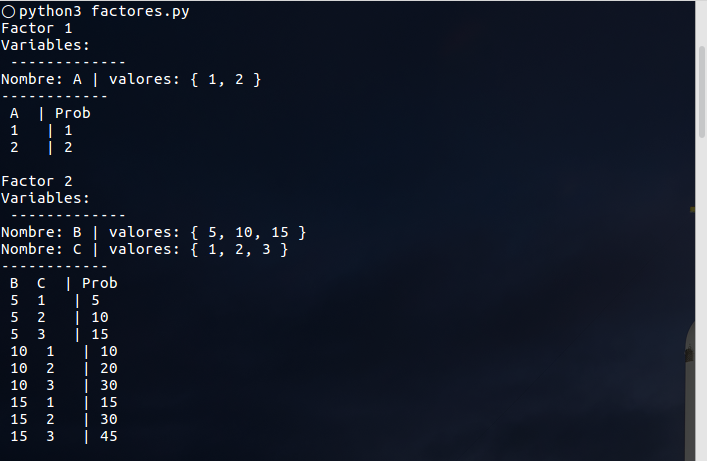
\includegraphics[scale=0.28]{factores/screen1.png}
    \caption{Creación de factores f1 y f2}
  \end{subfigure}
  ~
  \begin{subfigure}[b]{.45\textwidth}
    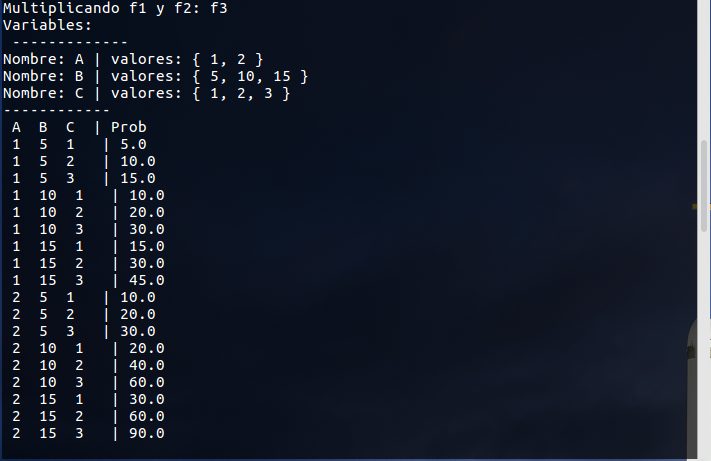
\includegraphics[scale=0.28]{factores/screen2.png}
    \caption{Multiplicando f1 y f2, para obtener f3}
  \end{subfigure}


  \begin{subfigure}[b]{.45\textwidth}
    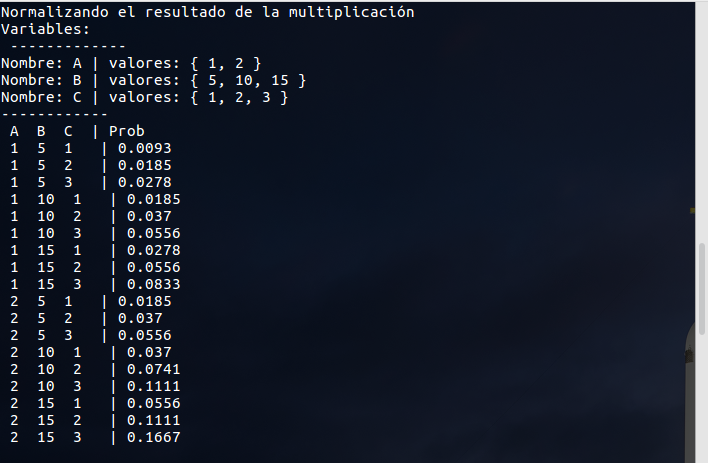
\includegraphics[scale=0.28]{factores/screen3.png}
    \caption{Normalizando f3}
  \end{subfigure}
  ~
  \begin{subfigure}[b]{.45\textwidth}
    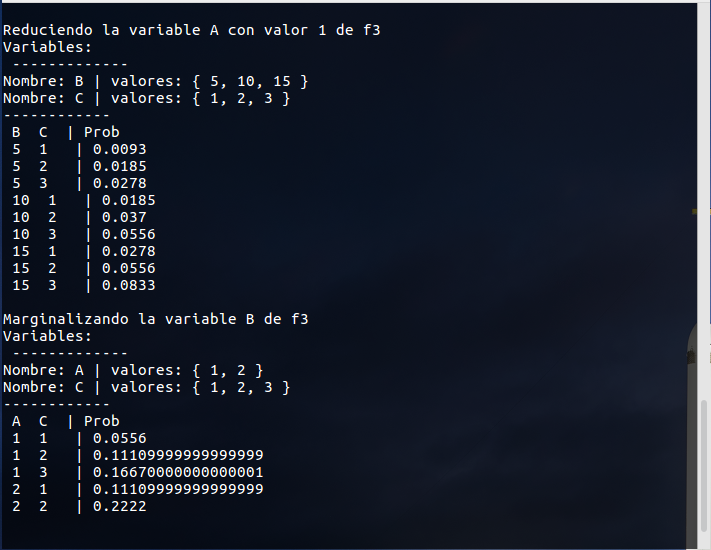
\includegraphics[scale=0.28]{factores/screen4.png}
    \caption{Reduciendo y marginalizando}
  \end{subfigure}
  \caption{Ejecución del código solución: crea dos factores, los multiplica, normaliza, reduce y marginaliza}
  \label{fig:P5solution}
\end{figure}

No olviden documentar y comentar su código.




\chapter[Inferencia]{Inferencias en Redes de Bayes usando factores}
\chapterauthor{Verónica Esther Arriola Ríos}

%----------------------------------------------------------------------------------------
% Aplicaciones de la clase Factor
%----------------------------------------------------------------------------------------

Esta práctica es un pequeño complemento a la práctica \emph{Factores}.

\section{Objetivo}

El alumno utilizará la clase factor para resolver consultas a una red de Bayes.

\begin{compactitem}
 \item Que el alumno identifique las ventajas de utilizar factores para calcular distribuciones de probabilidad sobre realizar los cálculos en la forma tradicional: con sumas y productos, considerando cada valor posible manualmente.
 
 \item Identificar la relación entre marginalización en probabilidad y marginalización de factores.
 
 \item Combinar las operaciones reducción y normalización de factores para calcular la reducción en distribuciones de probabilidad.
 
 \item Que alumno pueda mapear de una ecuación con sumas y productos de distribuciones a las operaciones correspondientes con factores.
\end{compactitem}


\section{Introducción}

Para realizar esta práctica se tomarán ejemplos del problema de la fiesta de Pedro, por lo que necesitarás la gráfica obtenida y las distribuciones de probabilidad completadas en teoría. [\fref{Fig:GrafPedro}]

\begin{figure}
 \centering
 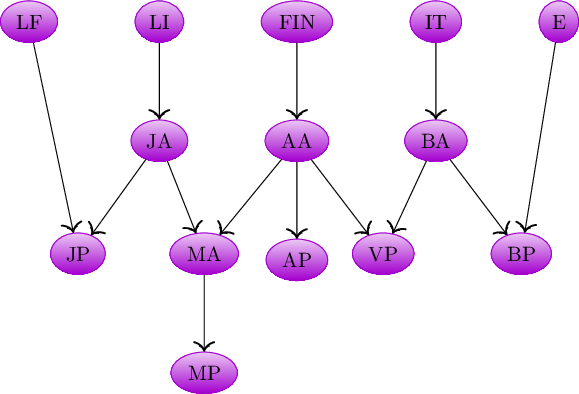
\includegraphics[width=0.8\textwidth]{inferenciasfactor/ComplicadaPedro.png}
 \caption{Gráfica con las relaciones de dependencia condicional del problema de la Fiesta de Pedro.  El significado de los nodos y las distribuciones de probabilidad correspondientes se pueden encontrar entre los textos del curso.}\label{Fig:GrafPedro}
\end{figure}


\section{Desarrollo}

Para resolver los ejercicios siguientes deberás utilizar la clase que programaste en la práctica Factores, por lo que será necesario que la entregues empaquetada en esta práctica también; si deseas hacer correcciones es un buen momento para incluirlas.

\subsection{Requisitos y resultados}

Para las instrucciones siguientes asumiremos que el código está en \code{Python}.  Si alguien decidió trabajar en otro lenguaje deberá consultar directamente con el ayudante del curso y adaptar las indicaciones a las convenciones del lenguaje elegido.

\begin{enumerate}
 \item Para esta práctica deberás entregar dos archivos:
 \begin{enumerate}
  \item \code{Factor.py}.  Es el código de la práctica anterior y será necesario para ejecutar esta.
  \item \code{PedroFactor.py}.  En este \textit{script} colocarás las funciones para resolver los problemas indicados.  Cada función que programes deberá:
  \begin{enumerate}
   \item Imprimir al inicio cuál es la \emph{consulta} (probabilidad) que está realizando.
   \item Los factores con resultados intermedios relevantes.  Antes de imprimir el factor, imprime su significado.  Por ejemplo: $P(ma|AP,VP)$, $P(MA,mp)$ ó $P(MA,JA)P(LI|bp)$.
   \item El resultado final, igualmente con algún formato que lo haga resaltar de las demás operaciones.
  \end{enumerate}
  Al final, en la sección \code{if \_\_name\_\_=='\_\_main\_\_':} mandar ejecutar todas las funciones mostrando tus resultados para cada ejercicio.
 \end{enumerate}
\end{enumerate}

\textbf{Notación:} Para abreviar sumas/marginalizaciones sucesivas, se utilizará la siguiente abreviatura:
\begin{align*}
 \sum_{A,B,C} &= \sum_A \sum_B \sum_C f(A,B,C)
\end{align*}


Las tareas que debes realizar son las siguientes:
\begin{enumerate}
 \item Crea todas las variables correspondientes a las variables aleatorias de la fiesta de Pedro como variables globales del \textit{script}.
 
 \item Crea todos los factores correspondientes a las distribuciones de probabilidad, también como variables globales.
 
 \item Crea una función por cada ecuación, donde resuelvas directamente la traducción de las operaciones siguientes, en el orden en el que están especificadas.  Para cada versión imprime el número de renglones que tienen tus factores después de cada multiplicación y marginalización. Observa que, al final, todas deben dar el mismo resultado
 \begin{align}
  P(VP,BP) =& \sum_{AA,BA,FIN,IT,E} P(VP|AA,BA)P(BP|BA,E)P(AA|FIN) \\
            & P(BA|IT)P(FIN)P(IT)P(E) \nonumber \\
  P(VP,BP) =& \sum_{AA,BA} P(VP|AA,BA)\sum_E P(BP|BA,E)\sum_{FIN}P(AA|FIN) \\
            & \sum_{IT}P(BA|IT)P(FIN)P(IT)P(E) \nonumber \\
  P(VP,BP) =& \sum_{AA,BA} \left\lbrace P(VP|AA,BA) \left[\sum_{FIN}P(AA|FIN)P(FIN)\right] \right\rbrace \\
            & \left[\sum_E P(BP|BA,E)P(E)\right] \left[ \sum_{IT}P(BA|IT)P(IT) \right] \nonumber \\  
 \end{align}
 
 \item Calcula la probabilidad de que María, Alicia y Víctor estén en la fiesta $P(MP,AP,VP)$.
 
 \item Calcula la probabilidad de que haya llovido el día que enviaron la invitación dado que María y Alicia estuvieron presentes.  Para ello seguirás el método siguiente.
 Recuerda que, por definición de probabilidad condicional:
 \begin{align*}
   P(LI|mp,ap) &= \frac{P(LI,mp,ap)}{P(mp,ap)}
 \end{align*}
  
 \begin{enumerate}
  \item Calcula la ecuación correspondiente para obtener $P(LI,mp,ap)$ usando la regla de la cadena para redes de Bayes.  Factorízala según sea conveniente y escribe tu resultado en los comentarios de la función de python para este ejercicio.
  
  \item Utiliza tus factores para obtener el resultado correspondiente, pero antes de multiplicar y marginalizar, manda llamar la operación \code{reducir} sobre todos los factores que contengan a $MP$ y $AP$, de modo que sólo te quedes con los renglones donde $MP=mp$ y $AP=ap$.
  
  \item Normaliza tu resultado final, esta es la probabilidad que estabas buscando.
 \end{enumerate}


\end{enumerate}




\chapter[Bayes Ingenuo]{Clasificador Bayesiano Ingenuo y aplicación de la clase Factor}
\chapterauthor{Luis Alfredo Lizárraga Santos}

\section{Objetivo}
Que el alumno utilice probabilidad en una aplicación de la vida real: modelar las probabilidades de que dado un texto, se pueda determinar a qué etiqueta pertenece: Ciencia, Tecnología, Cultura, etc. \par

\section{Introducción} 

Tener la posibilidad de etiquetar un texto automáticamente permite que las empresas del ramo periodístico puedan hacer un mejor uso de sus activos humanos para generar notas de valor y no estar etiquetando manualmente cada nota que entregan sus corresponsales. Por otro lado, estas etiquetas permiten una búsqueda de noticias más acertada para el lector, ya que son palabras clave derivadas del texto de la noticia.

En esta práctica utilizaremos un algoritmo de Aprendizaje automático: el Clasificador Bayesiano Ingenuo (\textit{Naive Bayes Classifier}).

\subsection{Clasificador Bayesiano Ingenuo}

Una manera sencilla de obtener una etiqueta para cualquier texto es utilizar un Clasificador Bayesiano Ingenuo, el cual se basa en el uso de Probabilidad y el Teorema de Bayes para predecir la etiqueta para un texto dado, obteniendo la probabilidad de cada etiqueta y retornando la más probable. A continuación veremos un ejemplo de cómo aplicar este clasificador, basado en una entrada del blog de Monkey Learn \parencite{Stecanella2017}


\subsection{Utilizando un Clasificador Bayesiano}

Supongamos que queremos construir un clasificador que nos diga las etiquetas más probables para un texto y tenemos los siguientes datos de entrenamiento:

\begin{figure}[H]
  \begin{center}
    \begin{tabular}{ l | c }
      Texto & Etiqueta \\ \hline
      de acuerdo con el portal de datos abiertos de la ciudad de méxico & CDMX  \\ \hline
      el gobierno capitalino mejora la seguridad en ciudad de méxico & CDMX  \\ \hline
      claudia sheinbaum aseguró que no se elevarán las tarifas para los capitalinos & CDMX  \\ \hline
      clasificación a octavos de final de la champions league & Deportes\\ \hline
      la fifa determinó que deberá pagar seis millones de dólares & Deportes  \\ \hline
      con la oportunidad de clasificar a octavos, nápoles recibirá al rb salzburgo & Deportes  \\ \hline
      el presidente lamentó lo sucedido al alcalde de valle de chalco & Nacional  \\ \hline
      la comisión temporal de presupuesto del instituto nacional electoral & Nacional  \\ \hline
      por la mañana, durante su conferencia de prensa, el presidente & Nacional  \\
    \end{tabular}
  \end{center}
  \caption{Datos de entrenamiento}
\end{figure}

¿Cómo podríamos saber a qué etiqueta pertenece el texto \quotes{desde el aeropuerto capitalino fue trasladada}?

Por ser un clasificador Bayesiano, calcularemos la probabilidad de que el texto anterior tenga alguna de las etiquetas Deportes, Nacional o CDMX y tomaremos la más alta. Entonces, lo que buscamos obtener es
\[P( CDMX | x ), \ P( Nacional | x ), \ P( Deportes | x )\]
donde
\[x = desde \ el \ aeropuerto \ capitalino \ fue \ trasladada \]

\subsection{Propiedades}

Lo primero que debemos de hacer al crear un modelo de Aprendizaje Automático es definir qué propiedades se utilizarán para que nuestro algoritmo pueda determinar la etiqueta correcta. Una propiedad es un pedazo de información que se le da al algoritmo para que aprenda las correlaciones o patrones existentes. Un ejemplo de propiedades que se podrían utilizar si se quisiera saber si una persona es más propensa a consumir cervezas artesanales son: edad, sexo, nivel de ingreso, etc. y se excluirían datos que pueden no ser relevantes para el modelo como nombre, correo o si están casados.

Estas propiedades deben tener una representación numérica para que el algoritmo pueda entenderlas, pero en nuestro caso sólo tenemos texto. Para poder hacer cualquier tipo de cálculo primero debemos transformar el texto a una representación numérica, esto lo logramos utilizando frecuencias de palabras, nos fijamos en cuántas veces aparece cada palabra por etiqueta.

\subsection{Teorema de Bayes}

Para lograr calcular probabilidades sobre frecuencias de palabras, utilizaremos el Teorema de Bayes, el cual nos permite obtener una probabilidad condicional a partir de la probabilidad condicional invertida y sus componentes, como podemos ver en la fórmula:

\[ P( A | B ) = {{P( B | A ) \times P(A)} \over P(B)} \]

En nuestro caso, para calcular \(P( CDMX | x )\) esta fórmula se traduce a:

\[ P( CDMX | x ) = {{P( x | CDMX ) \times P(CDMX)} \over P(x)} \]

% Pero, como queremos saber qué etiqueta tiene mayor probabilidad, podemos igualar ambos lados, eliminar el divisor, y así solo comparamos 

% \[ {P(Un juego muy cerrado| CDMX) \times P(CDMX)} \]

% con

% \[ {P(Un juego muy cerrado| No deportes) \times P(No deportes)} \]

Para calcular fácilmente la probabilidad condicional \(P(x | CDMX)\), basta con que contemos el número de veces que aparece el texto \quotes{desde el aeropuerto capitalino fue trasladada} para cada una de las etiquetas. Aquí nos topamos con un problema... ¡el texto completo no aparece en ninguna de las etiquetas!.

\subsection{Clasificador ingenuo}

Un clasificador ingenuo es aquél que supone que las propiedades proporcionadas al algoritmo son independientes entre ellas, logrando hacerlo más robusto sobre pocos datos o datos mal etiquetados.
Utilizando este supuesto, nos permite tomar cada palabra del texto como propiedad, en lugar de tomar el texto completo. Podemos ver que: 

\[ P(x) = P(desde) \times P(el) \times P(aeropuerto) \times P(capitalino) \times P(fue) \times P(trasladado) \]

lo cual nos permite calcular la probabilidad condicional como
\[ P(x | CDMX) = P(desde|CDMX) \times P(el|CDMX) \times P(aeropuerto|CDMX) \]
\[ \times P(capitalino|CDMX) \times P(fue|CDMX) \times P(trasladado|CDMX) \]

facilitándonos el cálculo de esta probabilidad, ya que estas palabras aparecen una o varias veces en nuestro conjunto de entrenamiento.

\subsection{Calculando probabilidades}

Como habíamos mencionado, haremos un conteo de palabras y de etiquetas. Primero, calculamos la probabilidad \textit{a priori} de las etiquetas: \(P(CDMX) = {1 \over 3}\), \(P(Nacional) = {1 \over 3}\) y \(P(Deportes) = {1 \over 3}\). Después, para calcular \(P(desde|CDMX)\) debemos tomar el número de veces que aparece la palabra \quotes{desde} dentro de los textos con la etiqueta \quotes{CDMX} y lo dividimos entre el número de palabras totales con la etiqueta \quotes{CDMX}, pero podemos ver que \quotes{desde} no aparece dentro de los textos con la etiqueta de \quotes{CDMX}, lo cual nos arroja que \(P(desde|CDMX) = 0\), pero al hacer las multiplicaciones para determinar \(P(x| CDMX)\) causaría que la probabilidad del texto completo sea $0$ y se pierda información sobre las probabilidades.

Para resolver este problema se aplican técnicas de suavizado \parencite[ver][202]{ManningSchutze1999} como el suavizado de Laplace, sumando $1$ a cada dividendo y lo contrarrestamos sumando el número de palabras posibles sin repetirse a cada divisor, así tendríamos \(P(desde|CDMX) = {{0 + 1} \over {35 + 67} }\). Esto lo repetimos con cada palabra del texto \quotes{desde el aeropuerto capitalino fue trasladada} y con cada etiqueta, obteniendo las siguientes tablas:

\begin{figure}[H]
  \begin{center}
    \begin{tabular}{ l | c }
      X & $P(X|CDMX)$ \\ \hline
      desde & $0 + 1 \over {35 + 67}$ \\ \hline
      el & $2 + 1 \over {35 + 67}$ \\ \hline
      aeropuerto & $0 + 1 \over {35 + 67}$ \\ \hline
      capitalino & $2 + 1 \over {35 + 67}$ \\ \hline
      fue & $0 + 1 \over {35 + 67}$ \\ \hline
      trasladada & $0 + 1 \over {35 + 67}$ \\
    \end{tabular}
  \end{center}
\end{figure}

\begin{figure}[H]
  \begin{center}
    \begin{tabular}{ l | c }
      X & $P(X|Deportes)$ \\ \hline
      desde & $0 + 1 \over {31 + 67}$ \\ \hline
      el & $0 + 1 \over {31 + 67}$ \\ \hline
      aeropuerto & $0 + 1 \over {31 + 67}$ \\ \hline
      capitalino & $0 + 1 \over {31 + 67}$ \\ \hline
      fue & $0 + 1 \over {31 + 67}$ \\ \hline
      trasladada & $0 + 1 \over {31 + 67}$ \\
    \end{tabular}
  \end{center}
\end{figure}

\begin{figure}[H]
  \begin{center}
    \begin{tabular}{ l | c }
      X & $P(X|Nacional)$ \\ \hline
      desde & $0 + 1 \over {30 + 67}$ \\ \hline
      el & $2 + 1 \over {30 + 67}$ \\ \hline
      aeropuerto & $0 + 1 \over {30 + 67}$ \\ \hline
      capitalino & $0 + 1 \over {30 + 67}$ \\ \hline
      fue & $0 + 1 \over {30 + 67}$ \\ \hline
      trasladada & $0 + 1 \over {30 + 67}$ \\
    \end{tabular}
  \end{center}
\end{figure}

Ahora, multiplicamos todas las probabilidades y obtenemos que: 

\[ P(x | CDMX) = {1 \over 102} \times {3 \over 102} \times {1 \over 102} \times {3 \over 102} \times {1 \over 102} \times {1 \over 102} \]
\[ P(x | CDMX) = { 9 \over 11.26162419\times10^{11}} = 7.99174244\times10^{-12} \]

\[ P(x | Deportes) = {1 \over 98} \times {1 \over 98} \times {1 \over 98} \times {1 \over 98} \times {1 \over 98} \times {1 \over 98} \]
\[ P(x | Deportes) = { 1 \over 8.858423809\times10^{11} } = 1.128868997\times10^{-12} \]

\[ P(x | Nacional) = {1 \over 97} \times {3 \over 97} \times {1 \over 97} \times {1 \over 97} \times {1 \over 97} \times {1 \over 97} \]
\[ P(x | Nacional) = { 3 \over 8.329720049\times10^{11} } = 3.601561616\times10^{-12} \]


Con lo cual nuestro clasificador le otorga la etiqueta \textbf{CDMX} al texto \quotes{desde el aeropuerto capitalino fue trasladada} y la segunda etiqueta más probable sería \textbf{Nacional}.


\subsection{Mejorando el clasificador}

Una manera sencilla de mejorar la clasificación de los textos es quitando palabras vacías \textit{(stop words)}, donde una palabra vacía es aquella que \quotes{no aporta información al texto que está siendo procesado}\parencite[533]{ManningSchutze1999}. En cualquier lenguaje, estas palabras vacías sirven para proveer contexto a un texto, pero el Clasificador Bayesiano Ingenuo no hace uso del contexto para determinar las etiquetas pertenecientes a cada texto, entonces estas palabras sólo hacen más lento la obtención de etiquetas y pueden introducir falsos positivos en la clasificación. En este caso procederíamos a quitarlas de nuestros conjuntos de entrenamiento y prueba.

Utilizando las palabras vacías que define Alir3z4 en su repositorio de GitHub (https://github.com/Alir3z4/stop-words) en el ejemplo anterior, podemos ver que los datos de entrenamiento se reducen a

\begin{figure}[H]
  \begin{center}
    \begin{tabular}{ l | c }
      Texto & Etiqueta \\ \hline
      acuerdo portal datos abiertos ciudad méxico & CDMX  \\ \hline
      gobierno capitalino mejora seguridad ciudad méxico & CDMX  \\ \hline
      claudia sheinbaum aseguró elevarán tarifas capitalinos & CDMX  \\ \hline
      clasificación octavos final champions league & Deportes\\ \hline
      fifa determinó deberá pagar seis millones dólares & Deportes  \\ \hline
      oportunidad clasificar octavos, nápoles recibirá rb salzburgo & Deportes  \\ \hline
      presidente lamentó sucedido alcalde valle chalco & Nacional  \\ \hline
      comisión temporal presupuesto instituto nacional electoral & Nacional  \\ \hline
      mañana, durante conferencia prensa, presidente & Nacional  \\
    \end{tabular}
  \end{center}
  \caption{Datos de entrenamiento después de eliminar palabras vacías}
\end{figure}

Y nuestro texto a etiquetar quedaría así: \quotes{aeropuerto capitalino trasladada}. Entonces, haciendo los cálculos nuevamente, podemos ver que quedan de la siguiente manera

\begin{figure}[H]
  \begin{center}
    \begin{tabular}{ l | c }
      X & $P(X|CDMX)$ \\ \hline
      aeropuerto & $0 + 1 \over {18 + 51}$ \\ \hline
      capitalino & $2 + 1 \over {18 + 51}$ \\ \hline
      trasladada & $0 + 1 \over {18 + 51}$ \\
    \end{tabular}
  \end{center}
\end{figure}

\begin{figure}[H]
  \begin{center}
    \begin{tabular}{ l | c }
      X & $P(X|Deportes)$ \\ \hline
      aeropuerto & $0 + 1 \over {19 + 51}$ \\ \hline
      capitalino & $0 + 1 \over {19 + 51}$ \\ \hline
      trasladada & $0 + 1 \over {19 + 51}$ \\
    \end{tabular}
  \end{center}
\end{figure}

\begin{figure}[H]
  \begin{center}
    \begin{tabular}{ l | c }
      X & $P(X|Nacional)$ \\ \hline
      aeropuerto & $0 + 1 \over {17 + 51}$ \\ \hline
      capitalino & $0 + 1 \over {17 + 51}$ \\ \hline
      trasladada & $0 + 1 \over {17 + 51}$ \\
    \end{tabular}
  \end{center}
\end{figure}

Ahora, multiplicamos todas las probabilidades y obtenemos que: 

\[ P(x | CDMX) = {1 \over 69} \times {3 \over 69} \times {1 \over 69} \]
\[ P(x | CDMX) = { 3 \over 328509} = 0.000009132 \]

\[ P(x | Deportes) = {1 \over 70} \times {1 \over 70} \times {1 \over 70} \]
\[ P(x | Deportes) = { 1 \over 343000 } = 0.000002915 \]

\[ P(x | Nacional) = {1 \over 68} \times {1 \over 68} \times {1 \over 68} \]
\[ P(x | Nacional) = { 1 \over 314432 } = 0.00000318 \]

Con esto podemos ver que es más sencillo hacer las operaciones, obtenemos probabilidades de mayor magnitud por la disminución del número de palabras y las palabras restantes nos permiten una mayor exactitud en la determinación de las etiquetas.

\section{Desarrollo e implementaci\'on}

La práctica consiste en obtener el texto de las noticias proporcionadas por el feed RSS de Aristegui Noticias, separar las noticias en dos conjuntos: de entrenamiento y de prueba, eliminar las palabras vacías haciendo uso del repositorio de GitHub proporcionado anteriormente, entrenar un Clasificador Bayesiano Ingenuo con el primer conjunto y evaluar qué tan bien predice las etiquetas de las noticias del segundo conjunto. Para lograrlo deberán usar el ejemplo anterior como guía para obtener las probabilidades de cada etiqueta presente en la base de prueba y después comparar las etiquetas obtenidas por el clasificador contra las etiquetas reales.

Incluido en el apéndice~\ref{appe:auxiliar} se encuentra el archivo \classname{feed.db} que contiene al menos 50 notas con título, texto, tags y link con el siguiente formato:

\begin{minted}[mathescape,
               linenos,
               numbersep=5pt,
               gobble=2,
               frame=lines,
               framesep=2mm]{text}

    Title: ...
    Tags: ...
    Text: ...
    Link: ...

\end{minted}

Por ejemplo:

\begin{minted}[mathescape,
               linenos,
               breaklines,
               fontsize=\footnotesize,
               numbersep=5pt,
               gobble=2,
               frame=lines,
               framesep=2mm]{text}

    Title: Devolverá Senado 281 millones 537 mil 756 pesos a Hacienda
    Tags: MÉXICO, Poder Legislativo, Presupuesto, Secretaría de Hacienda y ...
    Text: El Senado de la República devolverá a la Tesorería de la Federación ...
    Link: https://aristeguinoticias.com/1401/mexico/devolvera-senado...

    Title: Consejeros y empleados del INE cobrarán lo mismo que en 2018 ...
    Tags: MÉXICO, INE, Justicia, Poder Judicial, Presupuesto
    Text: Una jueza federal permitió al Instituto Nacional Electoral (INE) ...
    Link: https://aristeguinoticias.com/1401/mexico/consejeros-y-empleados...

    Title: Buen inicio de semana del peso: dólar baja a 19 unidades
    Tags: Dinero y Economía, Estados Unidos, Finanzas, Peso Dólar
    Text: El peso mexicano tuvo este lunes un buen inicio de semana, ...
    Link: https://aristeguinoticias.com/1401/lomasdestacado/buen-inicio...

\end{minted}

Separen este archivo en dos para obtener una base de datos de entrenamiento y otra de prueba, procurando que la mayor parte de las noticias queden en la base de datos de entrenamiento.

Después deberán obtener el texto, el título y la etiqueta de cada noticia incluida en la base de datos de entrenamiento. Con esta información deberán calcular tres probabilidades, como se explica en el ejemplo visto en la sección anterior:

\begin{enumerate}
  \item La probabilidad de que se obtenga una etiqueta en específico:
  \begin{equation*}
   \#\ de\ veces\ que\ aparece\ la\ etiqueta \over \#\ total\ de\ muestras\ de\ etiquetas
  \end{equation*}
  
  \item La probabilidad de que se obtenga una palabra en específico:
  \begin{equation*}
   \#\ de\ veces\ que\ aparece\ una\ palabra \over \#\ total\ de\ muestras\ de\ palabras
  \end{equation*}
  
  \item La probabilidad de que una palabra aparezca en el texto de alguna etiqueta:
  \begin{equation*}
   P(palabra \mid etiqueta)
  \end{equation*}
\end{enumerate}

Podemos ver que terminaremos con tres variables aleatorias, las cuales debemos conservar en Factores para agilizar su consulta. Si tienen problemas obteniendo la probabilidad de que una palabra aparezca en el texto de alguna etiqueta les recomiendo lo siguiente: creen un diccionario de palabras por cada etiqueta, que contenga el número de veces que aparece cada palabra con la etiqueta dada y el número total de palabras por etiqueta.

Una vez que tengan sus probabilidades, habrán acabado con la fase de entrenamiento de su Clasificador Bayesiano Ingenuo. Solo faltaría evaluar qué tan bien predice las etiquetas de las noticias incluidas en su base de datos de prueba. Para esto, tendrán que determinar a qué etiqueta pertenece el texto de las noticias. Deberán proporcionar las 3 más probables, y comparar con las etiquetas reales imprimiendo ambos conjuntos de etiquetas lado a lado.

En el apéndice~\ref{appe:auxiliar} podrán encontrar un script auxiliar que obtiene las noticias y las guarda en la base de datos, que es un archivo de texto plano. Lo pueden utilizar para obtener bases de datos actualizadas.

\section{Requisitos y resultados}

Todo lo anterior lo deberán anexar a la carpeta de la práctica, listo para cargarlo y probarlo. En el \classname{readme} deben especificar cómo se ejecuta, cómo se cargan los archivos, etc. Tampoco olviden comentar su código.




\chapter{Cadenas de Márkov}
\chapterauthor{ %
  Benjamín Torres Saavedra \\
  Verónica Esther Arriola Ríos
}

%----------------------------------------------------------------------------------------
% Cadenas de Márkov
%----------------------------------------------------------------------------------------

En esta práctica se implementarán funciones para realizar cálculos básicos sobre cadenas de Márkov.

\section{Objetivo}

\begin{compactitem}
 \item Que el alumno se familiarice con los procesos estocásticos discretos denominados Cadenas de Márkov discretas y realice una implementación para resolver algunas de las preguntas más frecuentes que se pueden plantear sobre estos procesos.
\end{compactitem}


\section{Introducción}

Adicionalmente a lo visto en clase, que estuvo basado en el sitio de \hrefformat{https://www.gestiondeoperaciones.net/cadenas-de-markov/cadenas-de-markov-ejercicios-resueltos/}{Gestión de operaciones}, pueden consultar la página sobre cadenas de Márkov en \hrefformat{https://en.wikipedia.org/wiki/Markov_chain}{Wikipedia} así como algunos \hrefformat{https://en.wikipedia.org/wiki/Examples_of_Markov_chains}{ejemplos} sencillos.


\section{Desarrollo}

Para esta práctica se requiere implementar una clase para trabajar con cadenas de Márkov.  Se recomienda programarla en \code{Python}, ya que la biblioteca \code{numpy} contiene métodos para trabajar con matrices y vectores, lo cual simplifica mucho los puntos siguientes.  También se recomienda utilizar matrices columna para representar vectores, de esta manera funcionarán correctamente las multiplicaciones de matriz por vector.

La clase \code{CadenaDeMarkov} debe contener:

\begin{enumerate}
 \item Un constructor que reciba como parámetros:
 \begin{enumerate}
  \item Una lista con los nombres los estados posibles.
  \item Un vector con la probabilidad de iniciar en cada uno de los estados posibles.
  \item Una matriz de probabilidades, con la probabilidad de transitar de cada estado hacia los demás.
 \end{enumerate}

 \item Un método para generar una secuencia de estados a partir del modelo de Márkov iniciado dado el número $n$ de elementos que tendrá la secuencia; opcionalmente puede recibir como parámetro una semilla para la generación de números aleatorios.
 
 Para generar esta muestra necesitarás calcular los vectores con las distribuciones de probabilidad para $n$ pasos.  Dada cada distribución, utiliza un número aleatorio para determinar cuál de los estados corresponderá a ese paso.
 
 Devuelve una lista con la secuencia de estados.
 
 \item Obtener la probabilidad de una cadena de estados (punto extra si se permite que esta cadena tenga estados indeterminados).  Observa que esta es la distribución de probabilidad conjunta $P(S_0=s_0,S_1=s_1,...,S_n=s_n)$, escrito de otra forma, $P(s_0,s_1,...,s_n)$.  Deberá recibir como parámetro una lista con la secuencia de estados y devolver la probabilidad.
 
 \item Estimar las probabilidades a largo plazo de cada uno de los estados, es decir, la distribución límite, cuando sea posible.  Este método deberá devolver el vector con la distribución de probabilidades.
 
 \item Agregar un archivo donde se utilice tu clase para resolver un ejemplo, usando cada uno de los métodos.  Puedes usar algún ejemplo del sitio de gestión de operaciones.
\end{enumerate}


\subsection{Requisitos y resultados}

En una carpeta, dentro de un archivo comprimido incluir:

\begin{enumerate}
 \item El archivo de la clase \code{CadenaDeMarkov}.
 \item El archivo con el demo de prueba.
\end{enumerate}





\chapter{Algoritmos Genéticos}
\chapterauthor{Rodrigo Eduardo Colín Rivera}

% TODO Cambiar a párrafos las subsecciones que no se ven bien


\section{Objetivo}
Conocer el funcionamiento de los algoritmos genéticos, su aplicación, pros y contras.\par
Entender los mecanismos de herencia, mutación, selección y cruza, así como su relación con la selección natural.
Implementar un algoritmo genético que resuelva y optimice un problema dado.

\section{Introducci\'on}

Un algoritmo genético es una heurística de búsqueda que está basada en el proceso de \textbf{selección natural}.  Su objetivo es encontrar soluciones óptimas a problemas combinatorios. La selección natural es un proceso gradual mediante el cual las características biológicas se vuelven más o menos comunes en una población. Esto depende de las características heredadas y de la diferencia de éxito reproductivo de los organismos que interactúan con su entorno. La selección natural es el mecanismo clave de la \textbf{evolución}. El término de “selección natural” fue popularizado por Charles Darwin desde el año de 1859.

\section{Metodolog\'ia}

En un algoritmo genético, una \textbf{población} de candidatos a solución (también llamados \textbf{individuos} o fenotipos) es evolucionada para obtener soluciones óptimas del problema. Cada individuo tiene una representación (sus cromosomas o genotipo) que puede ser alterada o mutada; tradicionalmente, las representaciones son cadenas binarias de 0’s y 1’s, pero otras representaciones son posibles.\par

La evolución es un proceso iterativo mediante el cual se generan individuos aleatoriamente para crear otra población en cada iteración, llamada \textbf{generación}. En cada generación, la \textbf{aptitud} (\textit{fitness}) de cada individuo es evaluada. Usualmente la aptitud es el valor de la función objetivo del problema de optimización que se quiere resolver. Se seleccionan de manera aleatoria individuos de la población para que modifiquen su genoma, \textbf{recombinando} y posiblemente \textbf{mutando} aleatoriamente sus componentes para formar una nueva generación. La nueva generación de posibles soluciones es usada en la siguiente iteración del algoritmo. Comúnmente, el algoritmo termina cuando se alcanza el número máximo de iteraciones o el valor de aptitud de un individuo se ha aproximado lo suficiente a un valor óptimo.

\section{Requisitos del algoritmo gen\'etico}

\begin{enumerate}
  \item Una \textbf{representación} genética del dominio de la solución.
  \item Una \textbf{función de aptitud} (\textit{fitness}) a evaluar sobre el dominio de la solución.
\end{enumerate}

\noindent La representación estándar de cada individuo es un arreglo de bits, sin embargo, arreglos de otro tipo y estructuras funcionan esencialmente de la misma manera. El motivo por el cual se prefiere la representación estándar es porque facilita las operaciones de recombinación debido a la longitud fija del arreglo, también la operación de mutación se vuelve trivial como se notará más adelante.


\section{Componentes del algoritmo gen\'etico}

\subsection{Inicializaci\'on}

Usualmente se genera una cantidad de soluciones posibles de manera aleatoria para formar la población inicial. El tamaño de la población depende del problema y puede llegar a contener cientos de miles de individuos.

\subsection{Selecci\'on}

La selección es una etapa del algoritmo genético en la cual se selecciona un individuo de la población que después será recombinado con otro.\par

Existen diferentes maneras de realizar el proceso de selección, el más común es la \textbf{selección proporcional de aptitud} (selección de ruleta). En este tipo de selección, la aptitud (o \textit{fitness}) del individuo se asocia con su probabilidad de selección.\par

Entonces si \(f_i\)  es la aptitud del individuo \(i\) en la población, la probabilidad de ser seleccionado es:\par
\[p_i = {f_i \over \sum_{j=1}^{N} f_j}\]
donde \(N\) es el número de individuos en la población.\par

Esto es similar a imaginar una ruleta de casino. Usualmente una proporción de la rueda de la ruleta es asignada a cada posible individuo basado en su aptitud. Esto se logra al dividir la aptitud de cada individuo entre el total de aptitud de todos los individuos, que es equivalente a normalizarlos a 1. Entonces un individuo es aleatoriamente seleccionado de la manera en que lo haría una ruleta que está girando.

\subsection{Operadores gen\'eticos}

\subsubsection{Recombinaci\'on}

La recombinación es el operador genético que permite la variación de cromosomas de los individuos de la población de una generación a otra. Es análoga a la reproducción y la recombinación biológica. El proceso de recombinación consiste en tomar más de un individuo y producir un nuevo hijo o solución.\par

Hay varias técnicas de recombinación, la más habitual es la recombinación de un punto y consiste en seleccionar aleatoriamente un mismo punto de corte dentro de la cadena de cromosomas de los padres e intercambiar sus contenido para generar nuevos hijos:

\begin{figure}[H]
  \centering
  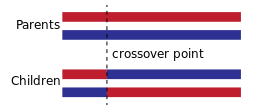
\includegraphics[scale=0.6]{geneticos/screen1.png}
  \caption{Operación genética recombinación de un punto.}
\end{figure}

\begin{table}[H]
  \centering
  \begin{tabular}{|l|l|}
  \hline
  Padre 1 & \textcolor{red}{1 1 0 1 0 0 1 0 0 1 1 0 1 1 0}                    \\ \hline
  Padre 2 & \textcolor{blue}{1 0 0 1 1 1 0 1 1 0 0 1 0 1 1}                   \\ \hline
  Hijo 1  & \textcolor{red}{1 1 0 1} \textcolor{blue}{ 1 1 0 1 1 0 0 1 0 1 1} \\ \hline
  Hijo 2  & \textcolor{blue}{1 0 0 1} \textcolor{red}{0 0 1 0 0 1 1 0 1 1 0}  \\ \hline
  \end{tabular}
  \caption{Ejemplo numérico de recombinación.}
\end{table}

\subsubsection{Mutaci\'on}

La mutación es el operador genético que mantiene la diversidad genética de una generación a otra, de manera análoga a la mutación biológica. La mutación altera uno o más de los genes (valores) en el cromosoma. Esta alteración puede cambiar por completo la solución antes de aplicar el operador de mutación y puede llegar a obtener mejores soluciones (o peores) dentro del algoritmo genético.\par

Las mutaciones ocurren valor por valor en un individuo de acuerdo a una probabilidad de mutación que es definida por el usuario. Esta probabilidad debería ser baja porque si se establece un probabilidad de mutación muy alta el algoritmo genético se convierte en una búsqueda de soluciones de manera aleatoria.

\begin{table}[H]
  \centering
  \begin{tabular}{|l|l|}
  \hline
  Cromosoma original & 1 1 0 1 \textcolor{red}{0} 0 1 0 0 1 1 0 1 \textcolor{red}{1} 0  \\ \hline
  Cromosoma mutado   & 1 1 0 1 \textcolor{red}{1} 0 1 0 0 1 1 0 1 \textcolor{red}{0} 0  \\ \hline
  \end{tabular}
  \caption{Ejemplo del operador de mutación.}
\end{table}

\subsection{Terminaci\'on del algoritmo}

Las iteraciones del algoritmo genético se terminan hasta que se alcanza alguna de las condiciones de terminación, que pueden ser:

\begin{itemize}
  \item Una solución es encontrada tal que satisface un criterio mínimo.
  \item Un número fijo de generaciones ha sido alcanzado.
  \item Se alcanza el máximo de los recursos posibles (por ejemplo: tiempo de procesamiento).
  \item Se alcanza el valor de aptitud más alto posible o se llega a un estado en el cual las iteraciones sucesivas no producen mejores resultados (puede deberse a la falta de diversidad, por ejemplo).
  \item Al hacer una inspección manual.
  \item O combinaciones de las anteriores.
\end{itemize}


\subsection{Variaciones}

\subsubsection{Elitismo}

Hay muchas variaciones que pueden hacerse a un algoritmo genético, una de ellas es el proceso de elitismo. Esta variante permite que algunas de las mejores soluciones pasen a la siguiente generación sin alteraciones por recombinación ni mutación.


\section{Desarrollo e implementaci\'on}

Se desea resolver el problema de las ocho reinas mediante algoritmos genéticos.  Este problema consiste en colocar ocho reinas del juego de ajedrez en un tablero de \(8 \times 8\) de tal manera que no se ataquen mutuamente. Entonces, encontrar una solución requiere que entre cualesquiera dos reinas no compartan columna, fila, ni diagonal entre ellas. El problema de las ocho reinas es un caso particular de otro más general, el de las \(n\)-reinas, que consiste en colocar \(n\) reinas en un tablero de dimensiones \(n \times n\).

\begin{figure}[H]
  \centering
  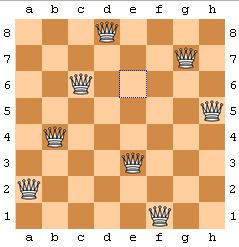
\includegraphics[scale=0.5]{geneticos/8queens.png}
  \caption{Ejemplo de solución al problema de las ocho reinas. \protect\footnotemark}
  \label{fig:queens}
\end{figure}
\footnotetext{https://matteoredaelli.wordpress.com/2009/01/05/n-queens-solution-with-erlang/}

\subsection{Consideraciones de la implementaci\'on}

\subsubsection{Representaci\'on gen\'etica}\par

Es recomendable emplear una representación de un tablero mediante una arreglo de números que identifica la posición por filas de cada reina.
Esta representación es muy conveniente porque evita que las reinas se ataquen por filas y facilita el proceso de encontrar una solución.

\begin{figure}[H]
  \centering
  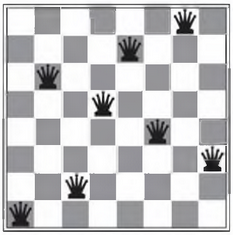
\includegraphics[scale=0.5]{geneticos/screen2.png}
  \caption{La representación del tablero sería [8, 3, 7, 4, 2, 5, 1, 6].}
  \label{fig:P8screen2}
\end{figure}


\subsubsection{Funci\'on de aptitud}\par

La optimización que se desea es encontrar un tablero en donde las reinas no se ataquen, de manera que la función de aptitud es inversamente proporcional a la cantidad de ataques entre reinas en un tablero.
La figura~\ref{fig:P8screen2} muestra un tablero donde sólo existe un ataque entre reinas, casi es un tablero óptimo por lo que el resultado de la función de aptitud debe ser un valor alto.

\subsubsection{Operador de recombinaci\'on}

Se utilizará el operador de corte de un punto eligiendo aleatoriamente un punto de corte, ilustrado con el siguiente ejemplo:

\begin{figure}[H]
  \centering
  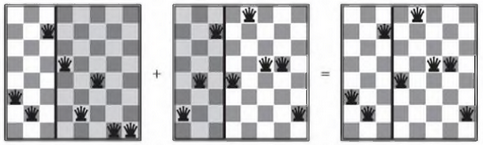
\includegraphics[scale=0.6]{geneticos/screen3.png}
  \caption{Recombinación de dos tableros para producir un nuevo tablero hijo.}
\end{figure}


\subsubsection{Operador de mutaci\'on}

El operador de mutación será definido con una probabilidad de mutación de 0.2. Es decir, se recorrerá cada gen del cromosoma (cada número del arreglo) y se modificará su valor con probabilidad 0.2.

\begin{table}[H]
  \centering
  \begin{tabular}{|l|l|}
  \hline
  Tablero original & {[} 8, 3, 7, 4, 2, \textcolor{red}{5}, 1, 6 {]}  \\ \hline
  Tablero mutado   & {[} 8, 3, 7, 4, 2, \textcolor{red}{3}, 1, 6 {]}  \\ \hline
  \end{tabular}
  \caption{Ejemplo de mutación para un tablero de ajedrez.}
\end{table}

\subsubsection{Selecci\'on}

Se utilizará el método proporcional de selección por ruleta descrito anteriormente.

\subsubsection{Terminaci\'on del algoritmo}

El algoritmo genético debe terminar cuando encuentra una solución óptima (sin ataques entre reinas) o cuando se hayan alcanzado 1000 generaciones.

\subsubsection{Cantidad de poblaci\'on}

La población de cada generación estará constituida por 50 individuos.

\subsubsection{Elitismo}

Para asegurarnos de mantener al menos una solución lo suficientemente buena, se utilizará elitismo de 1 individuo en cada generación.

\subsection{Pseudoc\'odigo}

El comportamiento general del algoritmo genético puede representarse a través del siguiente pseudocódigo:\medskip

\begin{algorithmic}
  \State $poblaci\acute{o}n\gets new Poblaci\acute{o}n(50)$
  \State $poblaci\acute{o}n.asignarAptitud()$
  \While{not $limiteDeGeneraciones$ or $\acute{o}ptimoEncontrado$}
    \State $nuevaPoblaci\acute{o}n.add(poblaci\acute{o}n.elitismo(1))$
    \While{not $nuevaPoblaci\acute{o}n.llena$}
      \State $individuo1\gets poblaci\acute{o}n.seleccionRuleta()$
      \State $individuo2\gets poblaci\acute{o}n.seleccionRuleta()$
      \State $hijo\gets recombinaci\acute{o}n(individuo1, individuo2)$
      \State $hijo.mutaci\acute{o}n()$
      \State $nuevaPoblaci\acute{o}n.add(hijo)$
    \EndWhile
    \State $poblaci\acute{o}n\gets nuevaPoblaci\acute{o}n$
    \State $poblaci\acute{o}n.asignarAptitud()$
  \EndWhile
  \State $print(poblaci\acute{o}n.mejorIndividuo())$
\end{algorithmic}

\section{Requisitos y resultados}

La implementación debe mostrar cada 50 generaciones el mejor individuo encontrado y mostrar la solución óptima una vez terminado el algoritmo.

\begin{figure}[H]
  \centering
  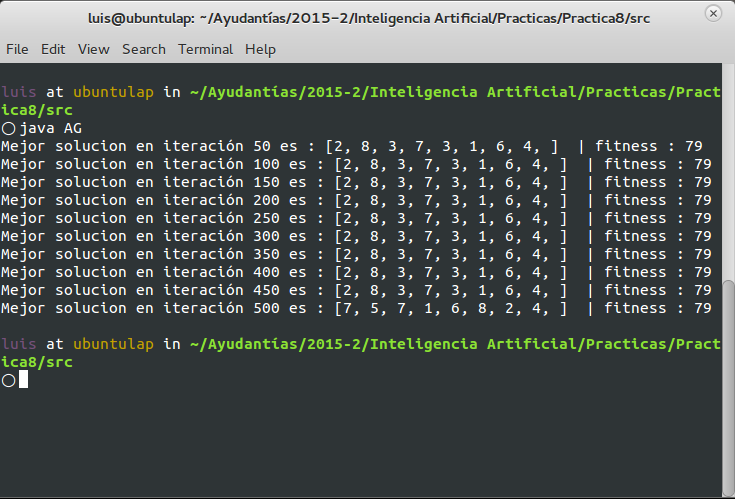
\includegraphics[scale=0.4]{geneticos/screen4.png}
  \caption{Ejemplo de resultado del algoritmo genético, donde se llegó al límite de generaciones.}
\end{figure}

\begin{figure}[H]
  \centering
  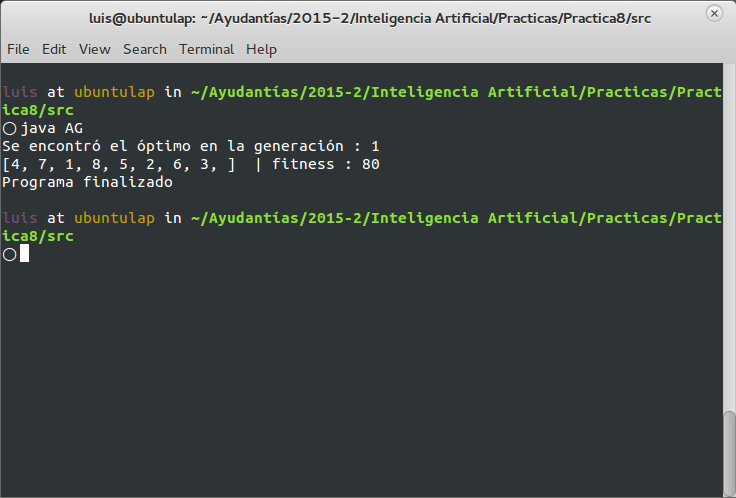
\includegraphics[scale=0.4]{geneticos/screen5.png}
  \caption{Ejemplo de resultado del algoritmo genético, donde se encontró una solución antes de llegar al límite de generaciones.}
\end{figure}


\noindent Lo podrán programar en \classname{Java} o \classname{Python}. No olviden comentar su código.\bigskip

\noindent \textbf{Punto Extra:} Si extienden su implementación para que pueda resolver el problema de $n$ reinas (tablero de $n \times n$) obtendrán un punto extra.


% \section{Agradecimientos}
% \noindent Esta práctica fue realizada originalmente por Rodrigo Eduardo Colín Rivera (animeroy@gmail.com). Se hicieron algunas modificaciones, pero sigue mereciendo crédito por su labor. \\\\





\chapter[Perceptrón]{Perceptrón, unidad fundamental de las redes neuronales}
\chapterauthor{Luis Alfredo Lizárraga Santos}


% \usepackage[linesnumbered,vlined]{algorithm2e}


\subsection{Objetivo}
Conocer el funcionamiento de las redes neuronales y lograr implementar un perceptrón simple que aprenda las operaciones \classname{AND} y \classname{OR}.

\subsection{Introducci\'on}

\quotes{Una red neuronal se puede definir como un modelo de razonamiento basado en el cerebro humano} \parencite[166]{Nengnevitsky2005}. Basándonos en el libro de Negnevisky explicaremos cómo funciona el cerebro, cómo las Redes Neuronales modelan el cerebro, cómo aprenden y finalizaremos con el Perceptrón \parencite[cap. 6]{Nengnevitsky2005}.


\subsection{Redes Neuronales Artificiales}

Sabemos que el cerebro consiste en un conjunto densamente interconectado de unidades básicas de procesamiento, llamadas neuronas. El cerebro humano contiene cerca de 86 mil millones de neuronas \parencite{Herculano-Houzel2009} y entre 100 y 500 billones de conexiones \parencite{Drachman2005}, llamadas \textbf{sinapsis}.\par

A pesar de que cada neurona tiene una estructura muy simple, un conjunto (aunque sea pequeño) de estos elementos constituye un poder de procesamiento enorme. Una neurona está constituida por un cuerpo celular, llamado \textbf{soma}, un conjunto de fibras llamadas \textbf{dendritas}, y una única fibra larga llamada \textbf{axón}. La figura~\ref{fig:P9screen1} representa dos neuronas conectadas.

Señales se propagan de una neurona a otra por medio de reacciones electroquímicas complejas. Substancias químicas que se liberan desde las sinapsis causan un cambio en el potencial eléctrico del cuerpo celular de la neurona. Cuando este potencial sobrepasa su umbral, una señal eléctrica, llamada \textbf{potencial de acción}, se manda a través del axón. Este pulso se dispersa y eventualmente llega a las sinapsis, haciendo que estas incrementen o decrementen su potencial. Pero el descubrimiento más interesante es que las neuronas exhiben \textbf{plasticidad}.\par

Esta plasticidad permite que las conexiones hacia las neuronas que conducen a la \quotes{respuesta correcta} se vean fortalecidas, mientras que las conexiones que llevan a la \quotes{respuesta equivocada} sean debilitadas. Como resultado, las redes neuronales tienen la habilidad de aprender mediante la experiencia.

\begin{figure}[h]
  \centering
  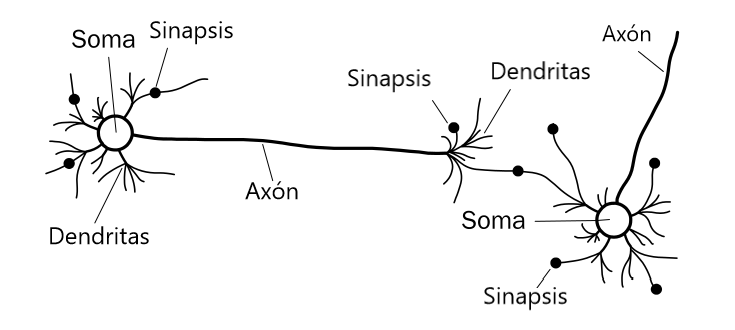
\includegraphics[scale=0.35]{perceptron/screen1.png}
  \caption{Partes de una neurona biológica. \parencite[166]{Nengnevitsky2005}}
  \label{fig:P9screen1}
\end{figure}

\subsubsection{¿C\'omo modelan al cerebro?}

\noindent Las neuronas de la red neuronal artificial se conectan entre sí usando conexiones con un peso dado, pasando señales de una neurona a otra. Cada neurona recibe un número de señales de entrada a través de sus conexiones, pero sólo produce una salida, como se muestra en la figura~\ref{fig:P9screen2}. Esta señal de salida se transmite por la conexión saliente de la neurona (lo equivalente al axón en la neurona biológica). Esta conexión saliente, a su vez, se separa en varias ramas que transmiten la misma señal. Estas ramas terminan como conexiones de entrada de otras neuronas en la red.

\subsubsection{¿C\'omo aprenden?}

\noindent Las neuronas se conectan mediante enlaces que tienen un peso asociado a ellos. Estos pesos son los medios para guardar información a largo plazo. Expresan la importancia de cada entrada de la neurona. Entonces, las redes neuronales \quotes{aprenden} por medio de ajustes a estos pesos.


\subsection{Neuronas Artificiales}

\begin{figure}[h]
  \centering
  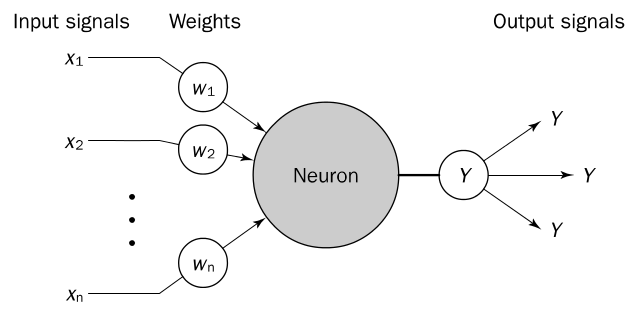
\includegraphics[scale=0.35]{perceptron/screen2.png}
  \caption{Diagrama de un perceptrón. \parencite[168]{Nengnevitsky2005}}
  \label{fig:P9screen2}
\end{figure}

\subsubsection{¿C\'omo se determina la salida?}

\noindent La neurona calcula la suma de las señales de entrada multiplicadas por el peso de su conexión con la neurona siguiente (combinador lineal) y compara este resultado con un umbral $\theta$. Si el total es menor que el umbral, la salida de la neurona es(\ -1)\ , si es mayor entonces la neurona se activa y su salida es (\ 1)\ . A lo descrito anteriormente se le llama función de activación.\par

Hay varias funciones que se pueden llegar a utilizar en lugar de esta, la figura~\ref{fig:screen3} presenta algunas de ellas.

\begin{figure}[h]
  \centering
  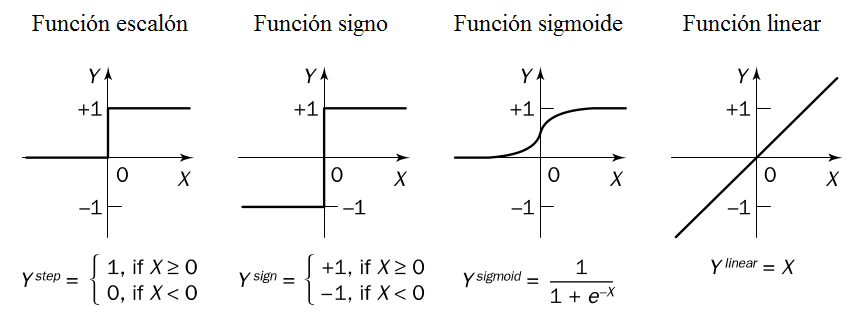
\includegraphics[scale=0.45]{perceptron/screen3-1.png}
  \caption{Ejemplos de funciones de activación de una neurona. \parencite[169]{Nengnevitsky2005}}
  \label{fig:screen3}
\end{figure}

\subsection{Perceptr\'on}

Un perceptrón es la forma más simple de una red neuronal, ya que representa a una sola neurona.

El perceptrón consiste en un combinador lineal seguido de una función de activación. Se le aplica la función umbral a la suma con pesos de las entradas menos el umbral, la cual produce una salida positiva si la suma es positiva, o una salida negativa si la suma es negativa. El objetivo del perceptrón es clasificar entradas en una de dos clases. Esto se expresa con la siguiente función: 

\[Y = f\left[\sum_{i=1}^{n}x_iw_i-\theta\right]\]
\parencite[169]{Nengnevitsky2005}

\subsubsection{Pero ¿c\'omo aprende a clasificar?}

Esto se logra haciendo pequeñas modificaciones a los pesos de las entradas para reducir las diferencias entre la salida obtenida y la salida deseada. El proceso de actualización de pesos es bastante simple. Como queremos obtener (o aproximarnos a) una salida deseada, tenemos que iterar sobre un conjunto de entrenamiento (de tamaño $m$) las veces necesarias, modificando los pesos de las conexiones, hasta minimizar el error en la salida. Si para el ejemplar de entrenamiento $j$, la salida es $Y(j)$ y la salida deseada es $Y_d(j)$, entonces la función de error está dada por:

\[ e(j) = Y_d(j)-Y(j)\]
\parencite[171]{Nengnevitsky2005}

Si $e(j)$ es positivo, se necesita incrementar $Y(j)$, pero si es negativo, se necesita disminuirlo. Tomando en cuenta que cada entrada contribuye \(x_i(j) \times w_i(j)\) a la entrada total $X(j)$, nos damos cuenta que si el valor de entrada $x_i(j)$ es positivo, aumentar su peso $w_i(j)$ incrementa la salida del perceptrón, mientras que si $x_i(j)$ es negativa, un aumento en su peso $w_i(j)$ disminuye el valor de salida del perceptrón. Por lo tanto se puede establecer la siguiente regla de aprendizaje:

\[w_i(j+1) = w_i(j) + \alpha \times x_i(j) \times e(j) \]
\parencite[171]{Nengnevitsky2005}

\noindent donde $\alpha$ es la \textbf{taza de aprendizaje}, una variable no negativa menor a $1$.

\subsection{Resumen del algoritmo de aprendizaje}

\noindent En pocas palabras, se necesitan cuatro pasos para que un perceptrón aprenda a clasificar las entradas \parencite[172]{Nengnevitsky2005}:\par

\begin{enumerate}
  \item \textbf{Inicialización:} Fijar los pesos iniciales \(w_1, w_2, ..., w_n\) y el umbral $\theta$ a números aleatorios en el rango $[-0.5, 0.5]$ (recomendado).
  \item \textbf{Activación:} Para un ejemplar $j$, activar el perceptrón aplicando las entradas\\ \(x_1(j), x_2(j), ..., x_n(j)\).
  \[Y(j) = f\left[\sum_{i=1}^{n}x_i(j)w_i(j)-\theta\right]\]
  donde $n$ es el número de entradas y $f$ es la función de activación.
  \item \textbf{Entrenamiento de pesos:} Se actualizan los pesos del perceptrón:
  \[w_i(t+1)=w_i(t)+\Delta w_i(t)\]
  donde \(\Delta w_i(t)\) es la corrección del peso al tiempo $t$ para el ejemplar $j$, que se calcula de la siguiente forma:
  \[\Delta w_i(t)=\alpha \times x_i(j) \times e(j)\]
  \item \textbf{Iteración:} Repetir el paso 2 y 3 para cada ejemplar del conjunto de entrenamiento hasta minimizar lo mejor posible el error. Si el resultado no es satisfactorio, continuar ejecutando otra vez desde el primer ejemplar.
  \label{algo:b}
\end{enumerate}

\subsection{Desarrollo e implementaci\'on}

\noindent Deberán crear dos perceptrones, uno que aprenda la operación \classname{AND} y otro la operación \classname{OR}, ambas de tres variables. Cada neurona tendrá cuatro entradas, tres para las entradas de la operación lógica y una para el sesgo.\par

\begin{figure}[H]
    \centering
    \begin{subfigure}[b]{0.4\textwidth}
        \centering
        \begin{tabular}{ l l c | r }
          $x_1$ & $x_2$ & $x_3$ & $Salida$\\ \hline
          0 & 0 & 0 & 0  \\ \hline
          0 & 0 & 1 & 0  \\ \hline
          0 & 1 & 0 & 0  \\ \hline
          0 & 1 & 1 & 0  \\ \hline
          1 & 0 & 0 & 0  \\ \hline
          1 & 0 & 1 & 0  \\ \hline
          1 & 1 & 0 & 0  \\ \hline
          1 & 1 & 1 & 1  \\
        \end{tabular}
        \caption{Operación AND}
    \end{subfigure}
    ~ 
    \begin{subfigure}[b]{0.4\textwidth}
        \centering
        \begin{tabular}{ l l c | r }
          $x_1$ & $x_2$ & $x_3$ & $Salida$\\ \hline
          0 & 0 & 0 & 0  \\ \hline
          0 & 0 & 1 & 1  \\ \hline
          0 & 1 & 0 & 1  \\ \hline
          0 & 1 & 1 & 1  \\ \hline
          1 & 0 & 0 & 1  \\ \hline
          1 & 0 & 1 & 1  \\ \hline
          1 & 1 & 0 & 1  \\ \hline
          1 & 1 & 1 & 1  \\
        \end{tabular}
        \caption{Operación OR}
    \end{subfigure}
\end{figure}

Su aplicación deberá permitir elegir distintos conjuntos de entrenamiento, en particular, tienen que especificar al menos 5 conjuntos de entrenamiento : 

\begin{enumerate}
  \item \texttt{[[0,0,0,0],[1,1,1,1]]} para AND y OR
  \item El conjunto que contenga todas las combinaciones posibles de entradas
  \item Y tres conjuntos más con elementos distintos, tomados de las tablas mostradas anteriormente.
\end{enumerate}

Con el formato: \[\texttt{[}x_1, x_2, x_3, Salida\texttt{]} \]

\noindent Esto para que se den una idea ustedes de lo importante que son los conjuntos de entrenamiento de un perceptrón.
También tienen que mostrar el proceso de entrenamiento, y una vez entrenado el perceptrón, debe permitir hacer consultas de estas operaciones lógicas.\par
Para probar su perceptrón, deberán utilizar el siguiente conjunto de entradas:

\[\texttt{[}\texttt{[}0,0,0\texttt{]}, \texttt{[}1,0,1\texttt{]}, \texttt{[}0,0,1\texttt{]}, \texttt{[}1,1,1\texttt{]} \texttt{]}\]

\noindent PD: Se les recomienda que no se compliquen y usen la función escalón (\textit{step function}) como función de activación.\par


\subsection{Requisitos y resultados}

Generen un reporte con observaciones de cómo se comporta el perceptrón con cada uno de los conjuntos de entrenamiento. Lo podrán programar en \classname{Java} o \classname{Python}. No olviden comentar su código.\medskip


% \begin{thebibliography}{1}

  % \bibitem{notes} Michael Nengnevitsky {\em Artificial Intelligence: A guide to Intelligent Systems}, 2005 :
  % Pearson Education Limited, Essex, England .

% \end{thebibliography}






%%
\part{Proyectos}



\chapter{STRIPS}
\chapterauthor{Verónica Esther Arriola Ríos}

%----------------------------------------------------------------------------------------
% STRIPS
%----------------------------------------------------------------------------------------

En este proyecto implementarás una pequeña máquina de inferencias utilizando los conocimientos
de la primera parte del curso.

\section{Meta}

El alumno experimentará de primera mano cómo programar los elementos escenciales de una
máquina de inferencias para un sistema experto.

\section{Objetivos}

\begin{compactitem}
 \item Que el alumno se familiarice con el uso del lenguaje de descripción PDDL para expresar
       los pormenores de un problema de planeación.
 \item Familiarizarse con el uso del diseño orientado a objetos en el código, para facilitar
       la implementación de los algoritmos que resolverán el problema de planeación.
 \item Que el alumno implemente un algoritmo de búsqueda que trabaje sobre objetos en un
       dominio PDDL.
 \item Que el alumno valore la relevancia del algoritmo de unificación, en un caso sencillo,
       para la identificación de acciones aplicables a un estado del dominio.
\end{compactitem}

\section{Desarrollo}

En este paquete se te entrega:
\begin{itemize}
 \item Una copia de la gramática BNF del lenguaje para descripción de problemas de planeación PDDL.
       No utilizarás todas las opciones que se incluyen, así que sólo revísala para que te des una 
       idea de lo que se puede hacer.
 \item Un script de \Python\ con la definición de las clases que representarán a los objetos en
       el dominio, hechos, acciones posibles, estado inicial y meta de un problema de planeación.
       Lee con cuidado la documentación.  Estas clases corresponden a los elementos de PDDL que
       vas a utilizar.  Observa que las clases listan los atributos, pero esta representación es
       independiente de la notación con paréntesis de PDDL.
 %\item En las notas del curso sobre STRIPS se reproduce un ejemplo tomado de \cite{Ghallab2004}.
\end{itemize}


\subsection{Escenario de prueba}

El programa que vas a realizar deberá poder resolver un pequeño problema de planeación, definido según la notación de PDDL.  El dominio siguiente se puede utilizar para probarlo.

\begin{lstlisting}[language=Lisp]
;; Especificación en PDDL1 de un dominio DWR simplificado
 
(define (domain platform-worker-robot)
  (:requirements :strips :typing)
  (:types
    contenedor
    pila	    ;tiene una base y una pila de contenedores.
    grúa	    ;sostiene máximo un contenedor.
  )
  (:predicates
    (sostiene ?k - grúa ?c - contenedor) ;la grúa ?k sostiene al contenedor ?c
    (libre ?k - grúa)                    ;la grúa ?k está libre
    (en ?c - contenedor ?p - pila)       ;el contenedor ?c está en la pila ?p
    (hasta_arriba ?c - contenedor ?p - pila) ;el contenedor ?c se encuentra hasta arriba de la pila ?p
    (sobre ?k1 - contenedor ?k2 - contenedor);el contenedor ?k1 está sobre el contenedor ?k2
  )
  ;; toma un contenedor de una pila con la grúa
  (:action toma
     :parameters (?k - grúa ?c - contenedor ?p - pila)
     :vars (?otro - contenedor)           ;variables locales (extra a PDDL)
     :precondition (and (libre ?k) (en ?c ?p) 
                       (hasta_arriba ?c ?p) (sobre ?c ?otro))
     :effect (and (sostiene ?k ?c) (hasta_arriba ?otro ?p)
                (not (en ?c ?p)) (not (hasta_arriba ?c ?p))
                (not (sobre ?c ?otro)) (not (libre ?k))))

  ;; pone al contenedor sostenido por la grúa en una pila
  (:action pon                                 
     :parameters (?k - grúa ?c - contenedor ?p - pila)
     :vars (?otro - contenedor)           ;variables locales
     :precondition (and (sostiene ?k ?c) (hasta_arriba ?otro ?p))
     :effect (and (en ?c ?p) (hasta_arriba ?c ?p) (sobre ?c ?otro)
                 (not (hasta_arriba ?otro ?p)) (not (sostiene ?k ?c))
                 (libre ?k))))
)
\end{lstlisting}

A continuación se incluye un ejemplar de problema.  Puedes diseñar otros tú y verificar que tu programa también los resuelva correctamente.

\begin{lstlisting}[language=Lisp]
;; un problema sencillo del dominio DWR simplificado
(define (problem dwrpb1)
  (:domain platform-worker-robot)

  (:objects
   k1 k2 - grúa
   p1 q1 p2 q2 - pila
   ca cb cc cd ce cf pallet - contenedor)

  (:init
   (en ca p1)
   (en cb p1)
   (en cc p1)

   (en cd q1)
   (en ce q1)
   (en cf q1)

   (sobre ca pallet)
   (sobre cb ca)
   (sobre cc cb)

   (sobre cd pallet)
   (sobre ce cd)
   (sobre cf ce)

   (hasta_arriba cc p1)
   (hasta_arriba cf q1)
   (hasta_arriba pallet p2)
   (hasta_arriba pallet q2)

   (libre k1)
   (libre k2))

   ;; el problema consiste en mover todos contenedores
   ;; ca y cc a la pila p2, los demás a q2
   (:goal
     (and (en ca p2)
          (en cb q2)
          (en cc p2)
          (en cd q2)
          (en ce q2)
          (en cf q2))
    )
)
\end{lstlisting}

\subsection{Tareas a realizar}

Las tareas que debes realizar son las siguientes:
\begin{enumerate}
\subsubsection{Parte I}
 \item Dibuja el estado inicial.  Puedes incluirlo como comentario en tu código como arte ASCII o adjuntar un archivo de imagen (no debe ser un archivo pesado).
 \item Crea a mano los objetos correspondientes al dominio y problema anteriores.
       Imprímelos y observa que todo esté correcto.
 \item Observa que el estado del mundo se representa como una lista de predictados aterrizados.
       Agrega el código necesario (clases o funciones) para que, dado un estado determine si una
       acción es aplicable o no y con qué sustitución (qué objeto se asigna a qué variable).
 \item Agrega el código para determinar si un estado satisface las condiciones indicadas en el 
       campo \emph{meta}.
\subsubsection{Parte II}
 \item Ahora agrega el código necesario para realizar una búsqueda en amplitud de la secuencia
       de acciones que se debe seguir para alcanzar la meta.  Haz que imprima lo que está
       haciendo de modo que puedas ver si se comporta como deseas.
 \item Utiliza tu programa para buscar una solución al problema anterior.
       ¿Es suficiente información? ¿Cómo se comporta tu programa?
\end{enumerate}



\chapter{Lego Mindstorms}
\chapterauthor{Luis Alfredo Lizárraga Santos}


\section{Objetivo}
\noindent Que el estudiante trabaje con un robot programable de tal forma que comprenda las funciones de distintos tipos de sensores y motores.

\section{Introducci\'on}

Se trabajará con Lego Mindstorms ya que es una plataforma fácil de usar y no es necesario tener conocimientos de circuitos digitales ni analógicos para la construcción del robot.

\subsection{¿Que es Lego Mindstorms?}

Lego Mindstorms es un paquete de software y hardware que permite crear robots programables, modulares y personalizables. Son caracterizados por contener una computadora central y módulos como: motores, actuadores, sensores de luz, de color, de presión, infrarrojos, etc. Y, como son Lego, se puede tener muchas configuraciones gracias a sus piezas intercambiables y construibles.


Ahora, para la práctica necesitaremos algunas cosas extras, ya que se utilizará el lenguaje de programación \classname{Python}, en lugar de usar la aplicación de diseño propia de Mindstorms. Se supondrá que se trabaja en Linux.

\subsection{Instalando ev3dev}

ev3dev es una distribución de Linux basada en Debian, lo cual permite tener una mayor disponibilidad de lenguajes y bibliotecas. La única desventaja es que sólo es compatible con la versión EV3 de Lego Mindstorms.

\noindent Se necesitará:

\begin{enumerate}
  \item El bloque programable de Mindstorms.
  \item Una memoria microSD con capacidad menor o igual a 32GB, preferentemente vacía ya que se borrarán todos los datos de esta.
  \item Una computadora con un adaptador para tarjetas microSD.
  \item Y una manera de comunicarse con el bloque programable, ya sea:
      \begin{itemize}
        \item Por un cable USB
        \item Por Wi-Fi usando un adaptador USB
        \item Por Ethernet usando un adaptador USB
        \item Por Bluetooth
      \end{itemize}
\end{enumerate}

\noindent Pueden obtener la imagen de ev3dev en: https://github.com/ev3dev/ev3dev/releases. Deben descargar la imagen que comienza con \quotes{ev3}, ya que las demás son para otros sistemas.

Una vez que tengan la imagen, procederemos a descomprimirla y copiarla a la memoria microSD:

\begin{enumerate}
  \item Abran una terminal y ejecuten el comando \classname{df} y guarden el resultado.
  \item Inserten la memoria y vuelven a ejecutar \classname{df} para obtener el nombre asignado por el sistema a su memoria.
  \item Desmonten la memoria, ejecutando \classname{sudo umount /dev/sdb1} (suponiendo que su memoria se encuentra en \classname{/dev/sdb1} ).
  \item Ahora, copiarán la imagen directamente a su memoria usando las aplicaciones \classname{dd} y \classname{xzcat}. Ejemplo: \classname{xzcat ~/Downloads/ev3dev-yyyy-mm-dd.img.xz | sudo dd bs=4M of=/dev/sdb}.
  \item Y por último, en cuanto termine la ejecución del paso anterior (puede demorar algunos minutos, no se desesperen), faltaría ejecutar \classname{sync} para asegurarse de que todas las escrituras al disco terminen y podrán remover la memoria microSD de su computadora.
\end{enumerate}


Después de haber descomprimido y escrito la imagen a la memoria, basta con insertarla al bloque programable y encenderlo.


\subsection{Conectándose a internet}

Para lograr una conexión a internet (y poder acceder al bloque por medio de \classname{ssh}), pueden consultar http://www.ev3dev.org/docs/getting-started/ donde encontrarán guías para cada método: por USB, usando un adaptador inalámbrico, usando un adaptador Ethernet USB o por bluetooth.


\subsection{Instalando Python, virtualenv y bibliotecas extras}

\subsubsection{¿Qué es virtualenv?}

Virtualenv es una aplicación que facilita hacer proyectos con Python, ya que crea un ambiente virtual en el que pueden utilizar una versión de Python específica, junto con \textit{add-ons} para esa versión, sin tener que utilizar esa misma versión globalmente. Léase: crea un contenedor con Python independiente.

\subsubsection{Instalación}
Una vez establecida una conexión por \classname{ssh} al bloque programable, basta ejecutar lo siguiente:

\begin{enumerate}
  \item \classname{apt-get update}
  \item \classname{apt-get install virtualenv virtualenvwrapper python-setuptools}\\ \classname{python-smbus python-pil}
  \item \classname{source /etc/bash\_completion.d/virtualenvwrapper}
  \item \classname{mkvirtualenv \{nombre del contenedor\} --python=/usr/bin/python2.7}\\ \classname{--system-site-packages}
  \item \classname{workon \{nombre del contenedor\}}
  \item \classname{easy\_install -U python-ev3}
\end{enumerate}

Con esto hecho, ya podrán acceder a los motores y sensores del EV3 desde Python, importando la biblioteca \classname{ev3}.\par

Para poder ejecutar su aplicación, pueden desarrollarla directamente desde el bloque programable usando \classname{vi} o \classname{nano}, pero se recomienda generar el archivo aparte y después copiarlo al bloque utilizando el comando \classname{scp}. Por ejemplo:

Suponemos que tenemos un archivo llamado \classname{seguidor\_de\_linea.py}, entonces ejecutamos:

\begin{itemize}
 \item \classname{scp seguidor\_de\_linea root@[dir\_ip\_bloque]:/home/robot}
\end{itemize}

Con esto, usando \classname{ssh}, nos dirigimos a la carpeta raíz del usuario y ejecutamos:

\begin{itemize}
 \item \classname{python seguidor\_de\_linea.py}
\end{itemize}

\section{Desarrollo e implementación}

Su práctica consiste en crear un robot seguidor de línea y un algoritmo para éste.

\subsection{Robot}

Pueden utilizar el sensor de color (para identificar la línea) y los distintos motores que tienen a su disposición. El diseño del robot es libre, un ejemplo de cómo montar los motores y sensor lo pueden ver en la figura~\ref{fig:P10robot}.

\subsection{Algoritmo}

Aquí tienen un ejemplo que utiliza dos motores (también lo pueden encontrar en el apéndice~\ref{appe:lego}), ubicados en los costados del bloque programable, y el sensor de color para ubicarse. Cabe notar que este algoritmo es bastante sencillo, ustedes deberán mejorarlo para que su robot siga la línea lo más fluidamente posible.

\begin{minted}[mathescape,
               linenos,
               numbersep=5pt,
               gobble=2,
               frame=lines,
               framesep=2mm]{python}
  from ev3.ev3dev import Motor
  from ev3.lego import ColorSensor

  a = Motor(port=Motor.PORT.A) # Abre el motor en el puerto A
  b = Motor(port=Motor.PORT.D) # Abre el motor en el puerto D
  sense = ColorSensor() # Abre el sensor para leer los valores
                        # que obtiene

  def move():
      maxSpeed = 100
      black = 10
      white = 78
      speedA = 50
      speedB = 50
      midpoint = (white-black)/2 + black
      tolerance = 20
      last_error = 0

      while True:
          # Obtiene el valor de reflectividad de la superficie
          # que ve el sensor
          val = sense.reflect 
          error = midpoint - val
          print error, val

          if abs(error) < tolerance:
              speedA = maxSpeed - last_error/2
              speedB = maxSpeed - last_error/2
              last_error = error
          else:
              if error > 0:
                  speedB = speedB + error/2
                  speedA = speedA - error/2
                  last_error = error
              else:
                  error = abs(error)
                  speedB = speedB - error/2
                  speedA = speedA + error/2
                  last_error = error

          if speedA < 0: speedA = 0
          if speedA > maxSpeed: speedA = maxSpeed
          if speedB < 0: speedB = 0
          if speedB > maxSpeed: speedB = maxSpeed

          # Hace que el motor A gire a la velocidad especificada
          # indefinidamente
          a.run_forever(speedA) 
          # Hace que el motor B gire a la velocidad especificada
          # indefinidamente
          b.run_forever(speedB) 
\end{minted}

Lamentablemente no hay mucha documentación sobre este plug-in, pero siempre pueden consultar más ejemplos en: https://github.com/topikachu/python-ev3

\section{Requisitos y resultados}

Deben entregar un script o aplicación que resuelva el problema de seguir una línea negra u obscura en un fondo contrastante junto con imágenes de la construcción del robot. Su script deberá ser lo más eficiente posible y debe guiar al robot a una velocidad mayor que el ejemplo que aparece en la sección anterior.


\begin{figure}[H]
  \begin{subfigure}{.5\textwidth}
    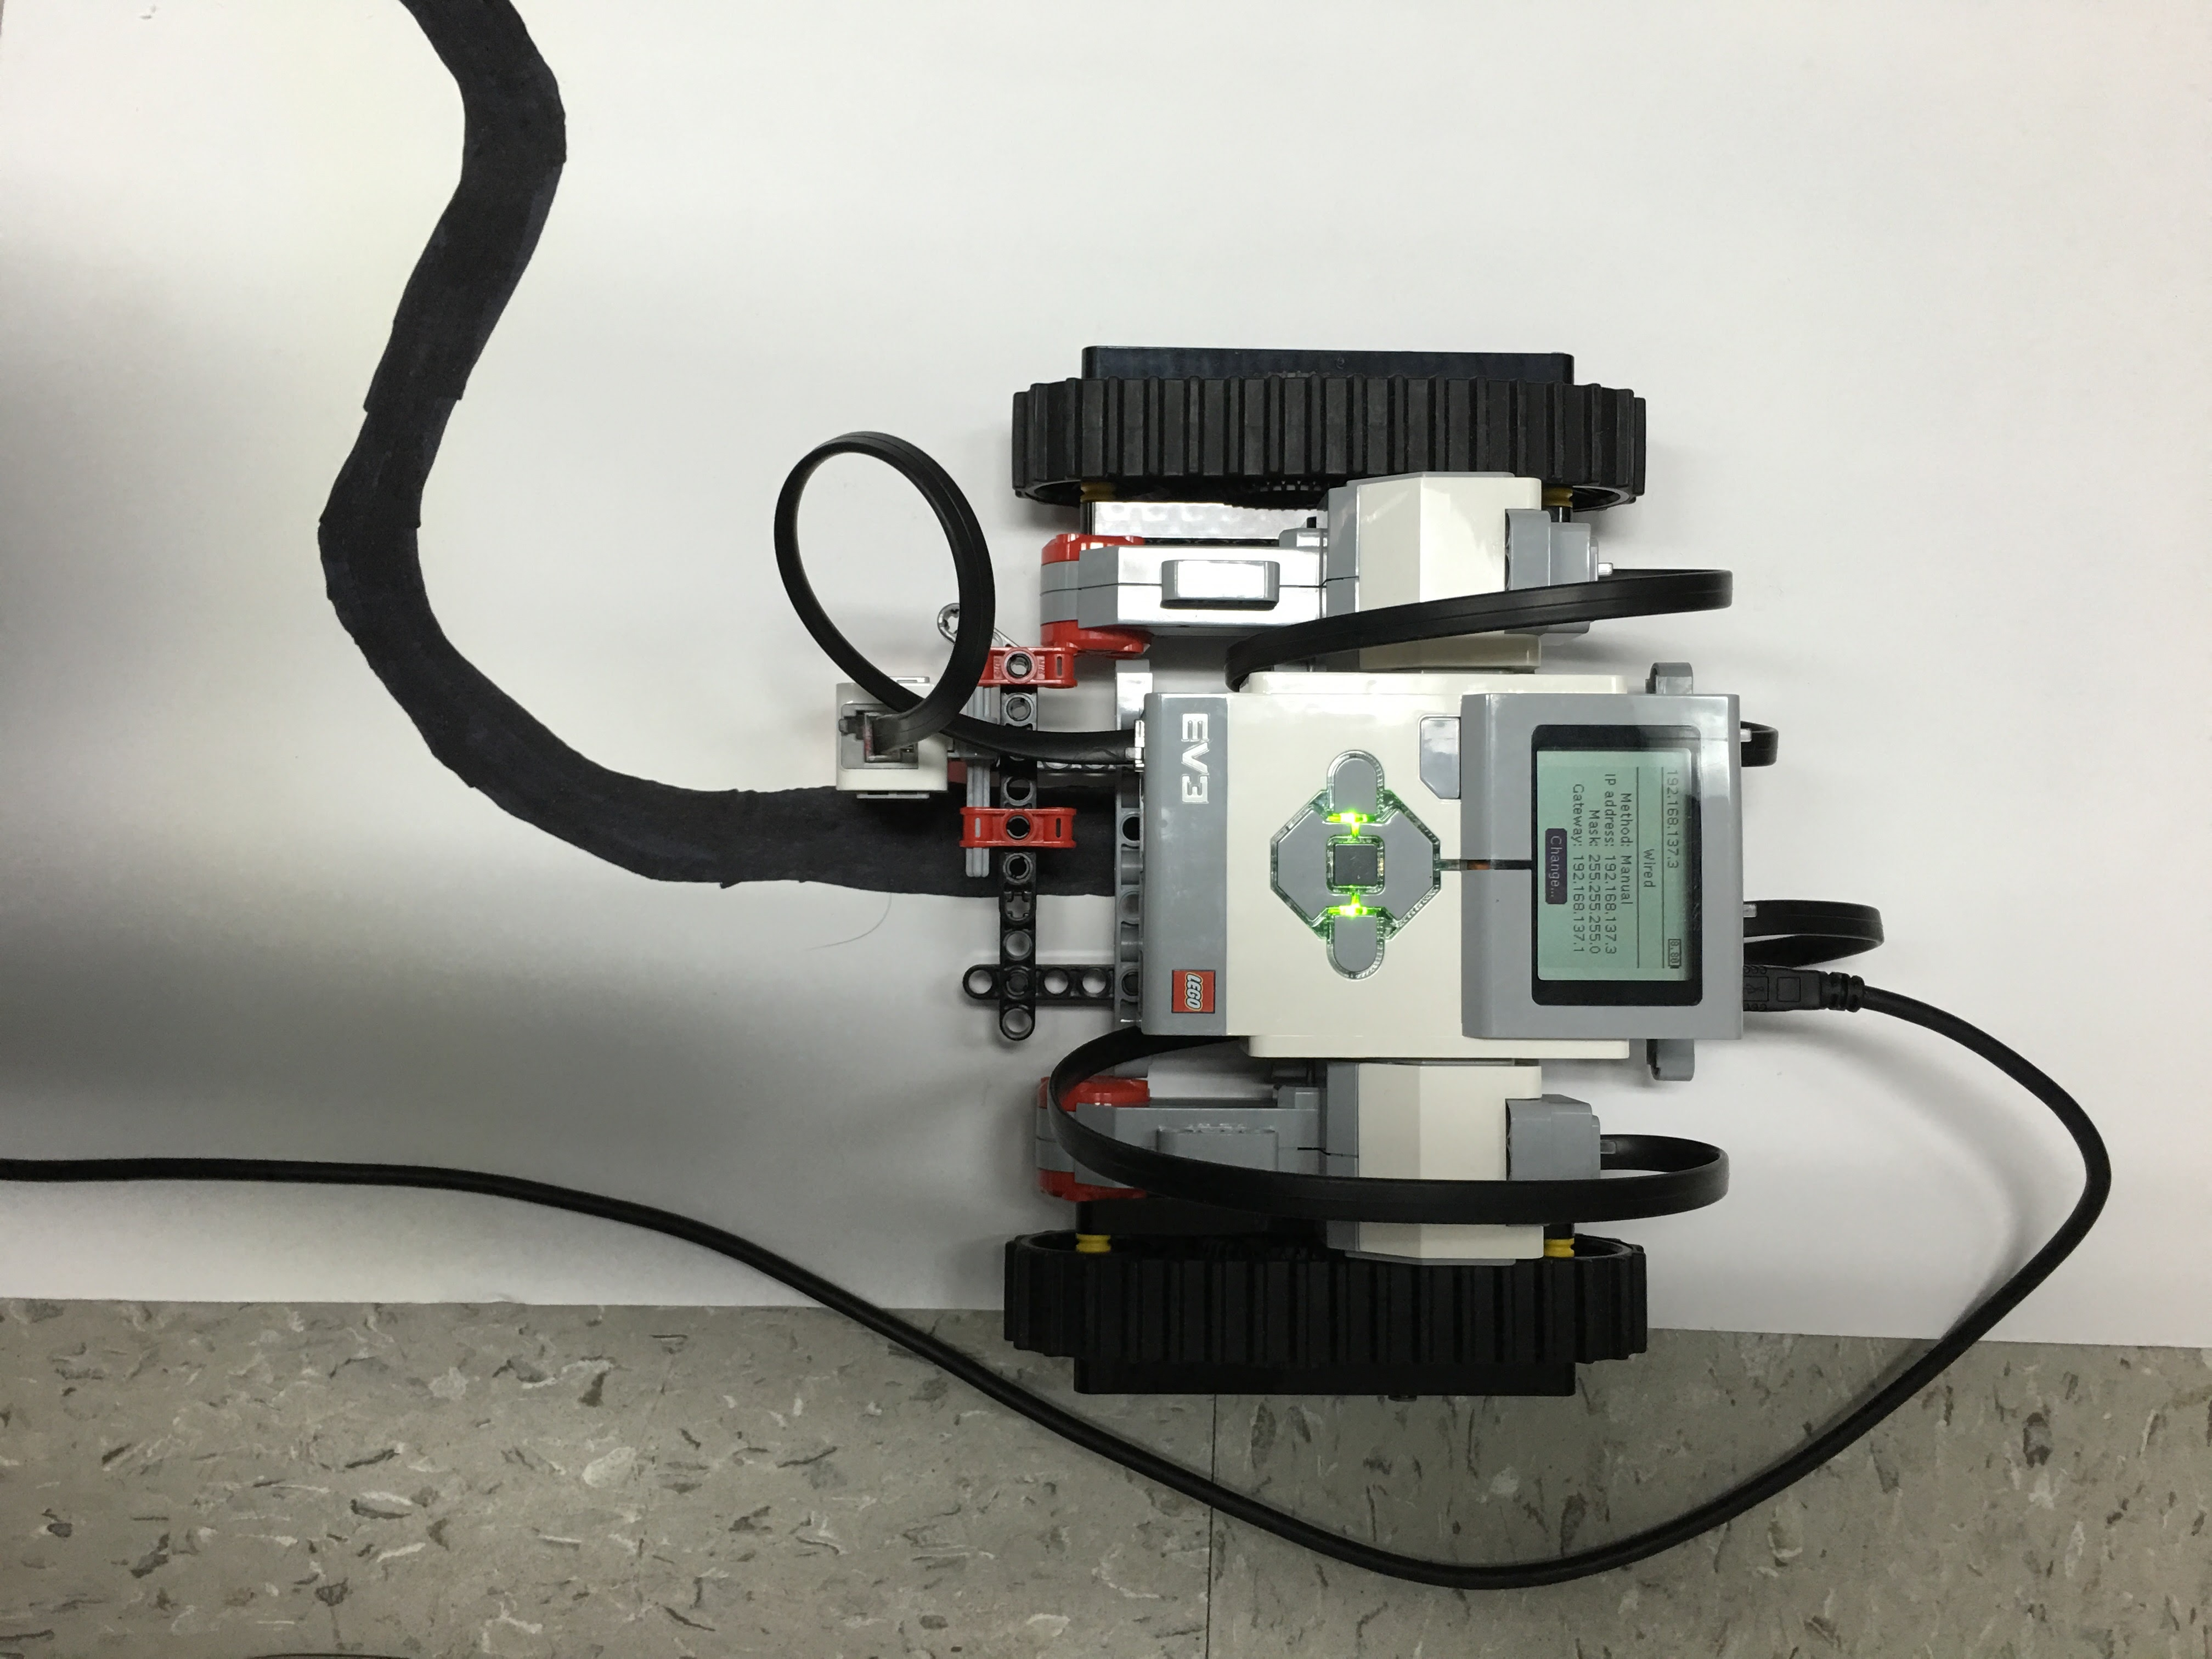
\includegraphics[scale=0.053]{legomindstorm/IMG_1892.JPG}
    % \includegraphics[width=.4\linewidth]{image1}
  \end{subfigure}
  \begin{subfigure}{.5\textwidth}
    % \includegraphics[width=.4\linewidth]{image1}
    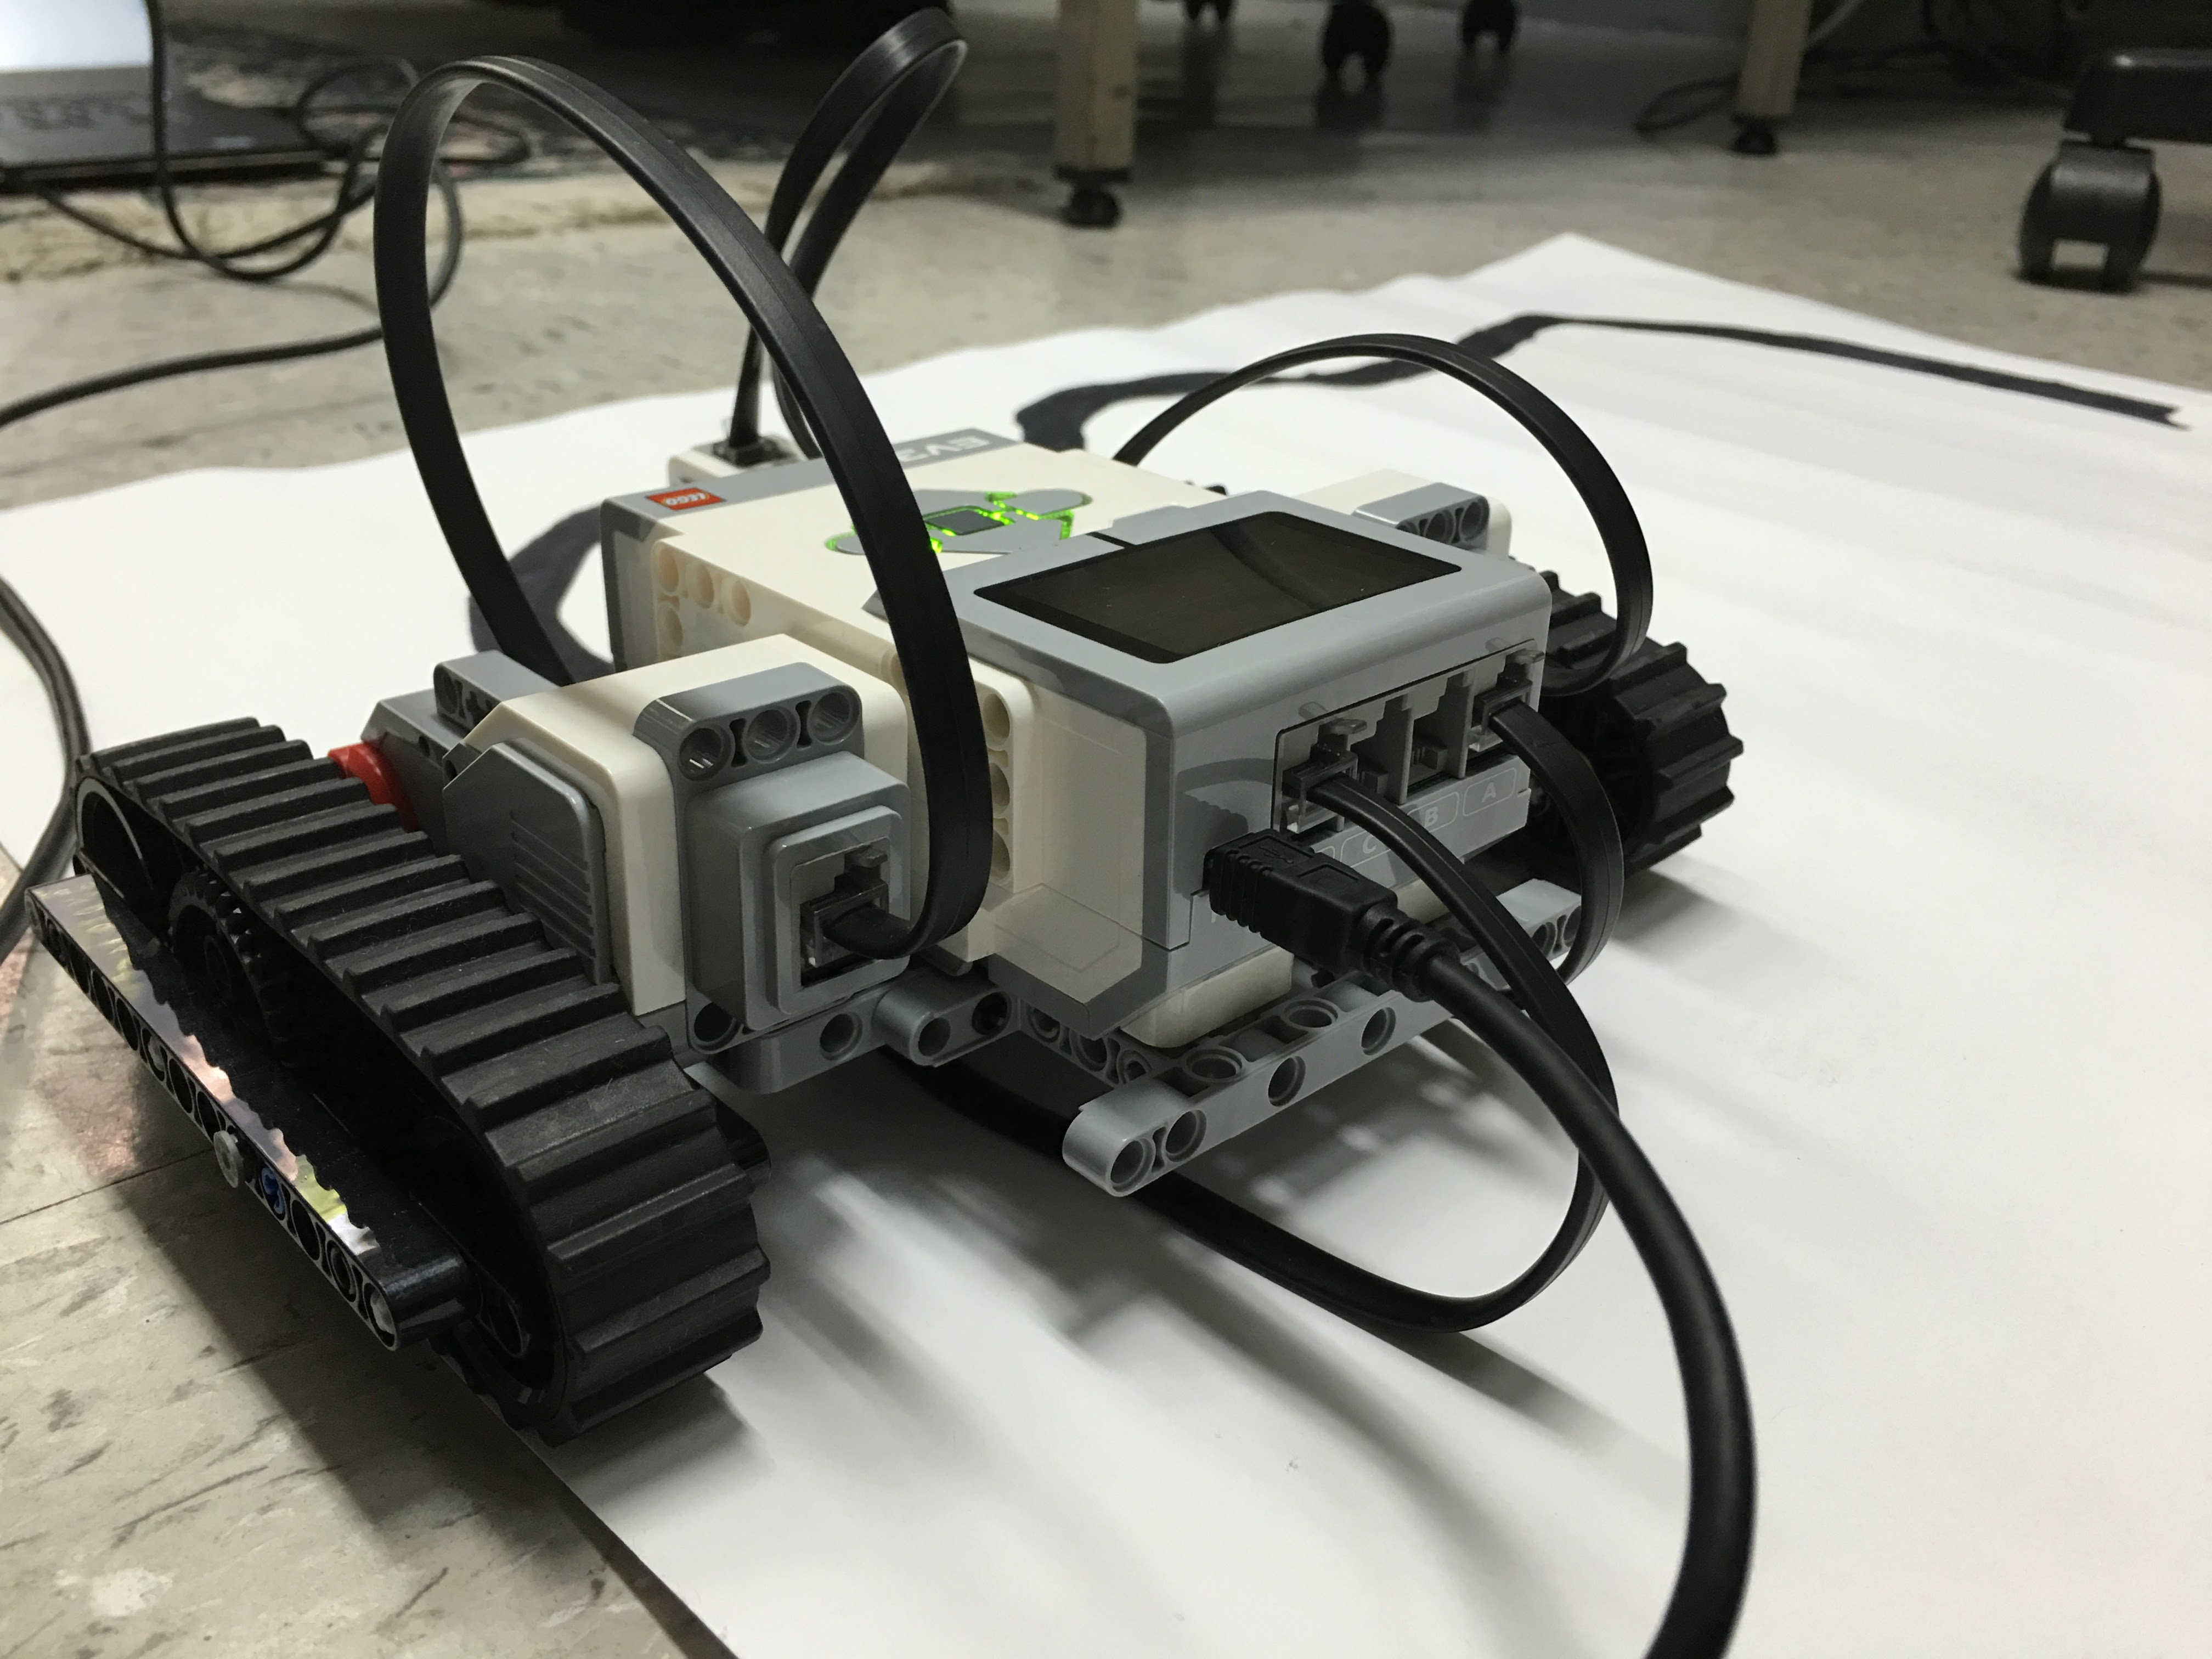
\includegraphics[scale=0.053]{legomindstorm/IMG_1895.JPG}
  \end{subfigure}
  \caption{Aquí se muestra una configuración ejemplo de robot seguidor de línea utilizando Lego Mindstroms.}
  \label{fig:P10robot}
\end{figure}

% \begin{thebibliography}{1}

  % \bibitem{notes} Michael Negnevitsky {\em Artificial Intelligence: A guide to Intelligent Systems}, 2005 :
  % Pearson Education Limited, Essex, England .

% \end{thebibliography}





\chapter{Localización de robots}
\chapterauthor{%
  Luis Alfredo Lizárraga Santos \\
  Verónica Esther Arriola Ríos
}

\subsection{Objetivo}
Conocer e implementar una técnica de localización utilizada en aplicaciones reales, específicamente para los robots \textit{Rhino} y \textit{Minerva} en los museos \textit{Deutsches Museum Bonn} y \textit{National Museum of American History}, respectivamente \parencite{Dieter1999}. Se utilizará Processing como herramienta de visualización de la técnica de localización.

\subsection{Introducci\'on}

\quotes{La localización robótica ha sido considerado como uno de los problemas fundamentales de la robótica. El objetivo de la localización es lograr estimar la posición del robot en un ambiente, apoyándose en un mapa de éste y con lecturas de sensores} \parencite{Dieter1999}. Tomando como base esta publicación de Dieter Fox, et. al. conoceremos los tipos de localización que existen y presentaremos la técnica que desarrolla la publicación: la localización de Markov.

\subsection{Localización Robótica}

Las técnicas que se han desarrollado hasta la fecha tratan de resolver uno de los dos tipos de localización que hay:

\begin{itemize}
  \item \textit{Localización local o rastreo.} Estas técnicas tratan de compensar errores odométricos durante el movimiento del robot. Son técnicas auxiliares que refinan la estimación que se tiene de la posición del robot en el entorno todo el tiempo, si la pierden es casi imposible volver a recuperarla \parencite{Dieter1999}.
  \item \textit{Localización global.} Estas técnicas están diseñadas para encontrar la posición estimada del robot globalmente, es decir, no es necesario tener un aproximado inicial de su posición. Estas técnicas pueden resolver el problema de localizar al robot al momento de encenderlo, al igual que permiten que se lleve al robot a una posición aleatoria del entorno durante su operación y recuperar su posición \parencite{Dieter1999}.
\end{itemize}

Como se podrán dar cuenta, las técnicas de localización global son más poderosas que las locales. Para esta práctica desarrollaremos una técnica de localización global de Markov.

\subsection{Localización de Markov}

La localización de Markov utiliza un sistema probabilístico que mantiene una distribución de probabilidad de la posición del robot sobre todo el entorno. Es decir, la probabilidad de que el robot se encuentre en cada posición del entorno en un tiempo dado. Por ejemplo, el robot puede iniciar con una distribución de probabilidad uniforme representando que no tiene idea de dónde se encuentra en el entorno, esto es, cada posición en el entorno tiene la misma probabilidad de que el robot se encuentre en ella. En el caso en el que el robot esté muy seguro de su posición, la distribución de probabilidad se convierte en una distribución unimodal centrada en la posición del robot.

\subsubsection{Ejemplo}

\begin{figure}
  \centering
  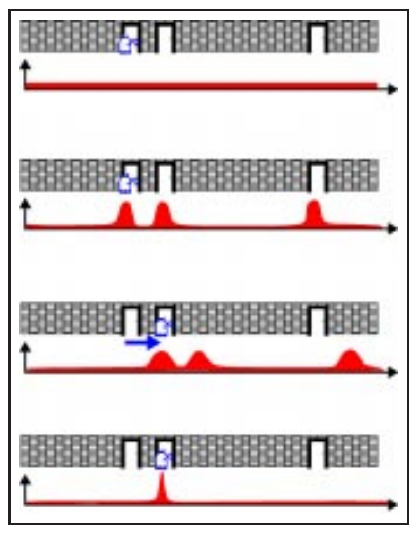
\includegraphics[scale=0.6]{localizacion/screen1.png}
  \caption{Ejemplo de localización de Markov. La gráfica de color rojo representa la distribución de probabilidad. \parencite{Dieter1999}}
  \label{fig:screen1}
\end{figure}


Estudiaremos el ejemplo sencillo que presentan Dieter Fox et. al. para ilustrar los conceptos de la localización de Markov.


Consideremos el entorno mostrado en la figura~\ref{fig:screen1}. Para simplificar, asumamos que el robot sólo puede moverse en una dimensión (enfrente-atrás). Ahora, supongamos que posicionamos el robot en algún lugar aleatorio del entorno, pero no le informamos al robot cuál es su posición. La localización de Markov representa este estado de \quotes{confusión} como una distribución de probabilidad uniforme sobre todo el conjunto de posibles posiciones del entorno, como lo muestra la primer gráfica de la figura~\ref{fig:screen1}. Asumamos que el robot hace una medición con sus sensores y determina que está al lado de una puerta. La localización de Markov modifica la distribución de probabilidad de tal manera que las posiciones que se encuentran a un lado de puertas tengan mayor probabilidad, esto queda ilustrado en la segunda gráfica de la figura~\ref{fig:screen1}. Notemos que la distribución resultante es multimodal(\footnote{Multimodal: Que tiene varios puntos máximos.} ), ya que la información obtenida por los sensores es insuficiente para determinar exactamente la posición del robot. También notemos que las posiciones que no se encuentran a un lado de una puerta aún tienen una probabilidad mayor que cero, esto es porque las mediciones de los sensores contienen ruido. Ahora, supongamos que el robot se mueve un metro hacia el frente. La localización de Markov incorpora este movimiento para que la distribución de probabilidad cambie como se representa en la tercer gráfica de la figura~\ref{fig:screen1}. Finalmente, asumamos que el robot vuelve a tomar una medición con sus sensores. Incorporando esta información a la obtenida anteriormente, vemos cómo la distribución de probabilidad cambia (cuarta gráfica de la figura~\ref{fig:screen1}) para asignar una alta probabilidad a la posición del robot, mientras que todas las demás posiciones tienen una probabilidad casi nula \parencite{Dieter1999}. 

\subsection{Desarrollo}

Tomando como base el modelo de Markov que presentan Dieter Fox et. al., el desarrollo de la práctica se dividirá en dos partes: la simulación del ambiente en donde se encuentra el robot y del robot, y la implementación del modelo en este ambiente.

\subsubsection{Simulación del ambiente y del robot}

\noindent Primero, iniciemos con el contenido y especificación del mundo en el cual se moverá el robot. Este mundo contendrá obstáculos y será rectangular (imagínense un cuarto o una oficina), las paredes serán obstáculos y cualquier otra cosa que se pueda encontrar en un cuarto u oficina normal: sillas, mesas, escritorios, etc. Será representado por una matriz de celdas, donde cada celda será cuadrada, podrá ser obstáculo o no y tendrá la longitud de un lado especificado en \(cm\). En la figura~\ref{fig:mapa} pueden apreciar un ejemplo de cómo se vería el mundo del robot representado gráficamente, donde los cuadros color café son obstáculos, el robot es el círculo verde y se muestra la orientación de este con una línea negra.

El robot podrá ocupar cualquier posición del plano de Processing \footnote{Cabe resaltar que para Processing el eje \(y\) se encuentra invertido, esto es, si aumentan el valor de \(y\) en el código, en la visualización esto se reflejará como si estuvieran caminando hacia abajo. }, no estará necesariamente en el centro de alguna celda. De hecho, se necesitará una función que, dada la posición del robot, nos permita saber dentro de qué celda se encuentra. Esta función nos será útil para la implementación del modelo de Markov discretizado.\par

\begin{figure}
  \centering
  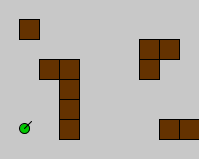
\includegraphics[scale=0.60]{localizacion/mapa.png}
  \caption{Representación visual del ambiente.}
  \label{fig:mapa}
\end{figure}

\paragraph{Movimiento del robot}

\noindent El robot podrá moverse libremente en el ambiente, salvo que se encuentre de frente un obstáculo, o los bordes del mundo ya que son considerados paredes. Este movimiento será controlado por el usuario, ya sea que utilicen las flechas direccionales de su teclado, alguna otra combinación de teclas, botones en la interfaz, o el mecanismo que ustedes prefieran. Lo importante es que el robot pueda moverse en línea recta y girar.\par

El usuario deberá poder especificar qué tanto se moverá el robot al momento de pulsar la tecla o botón requerido, ya sea si se desea cambiar de dirección o moverse en línea recta. Esto será muy importante, ya que necesitan saber la distancia real recorrida y la distancia real de giro para simular las medidas de los sensores.

\paragraph{Simulación de sensores}

\noindent Nuestro robot tendrá tres sensores:

\begin{enumerate}
  \item láser: mide la distancia desde el robot hacia el primer obstáculo en línea recta del sensor. El robot tendrá 8 de estos, ubicados cada \(45\degree\).
  \item odométrico: mide la distancia recorrida por el robot (en cm).
  \item de giro: mide el giro del robot en grados.
\end{enumerate}

Como se darán cuenta más adelante, utilizamos distribuciones Gaussianas para modelar las lecturas de los sensores. Cuando alguien busca armar un robot que tenga sensores, lo primero que debe hacer es calibrarlos para obtener un umbral de error inherente al sensor que se está utilizando para tenerlo en cuenta al momento de programar rutinas o desarrollar el software que permita al robot llegar a su objetivo. Si uno grafica las medidas obtenidas por el sensor versus la medida real, se llega a apreciar que forma una campana centrada en el valor de la medida real ya que los errores pequeños son comunes, pero errores grandes no tanto. Así nosotros podemos suponer que los sensores que estamos modelando generarán mediciones parecidas y utilizamos una distribución de probabilidad normal centrada en el valor real de lo que se mide para obtener la probabilidad de que el robot se encuentre en cierta posición dadas las mediciones recibidas.

\subparagraph{Láser}\medskip
En el caso de este sensor, las mediciones obtenidas pueden cambiar debido a los materiales donde se refleja el láser, entonces utilizaremos ruido gaussiano para simular este error.

Para cada sensor se necesitarán dos parámetros: la media (\( \mu_{laser} \)) y la desviación estándar (\( \sigma_{laser} \)). La desviación estándar es un parámetro que tú debes fijar, éste representa la cantidad de ruido que se introducirá a la medición. Y la media estará dada por la distancia real medida desde el robot hacia el primer obstáculo en línea recta en la dirección del sensor.

Para simular la medición del sensor con ruido, se hará lo siguiente:

\begin{enumerate}
  \item Obtener un número aleatorio utilizando \classname{nextGaussian()} de la clase\\ \classname{java.util.Random}.
  \item Multiplicar el número aleatorio obtenido por la desviación estándar (\( \sigma_{laser} \)).
  \item Sumar a la media (\( \mu_{laser} \)) el resultado anterior.
\end{enumerate}


\subparagraph{Odométrico}\medskip
La manera de simular la medición con ruido de éste sensor es casi idéntica al sensor láser, sólo que en lugar de medir la distancia hacia el obstáculo más cercano usaremos la distancia que el usuario proporcionó para mover al robot. Por ejemplo: Si el usuario decidió mover al robot \(10cm\), la media (\( \mu_{odometrico} \)) sería \(10cm\) y la desviación estándar (\( \sigma_{odometrico} \)) un parámetro especificado por ti.


\subparagraph{De giro}\medskip
Similarmente al sensor odométrico, la media (\( \mu_{de\ giro} \)) sería los grados reales girados y la desviación estándar (\( \sigma_{de\ giro} \)) un parámetro especificado por ti.

\subsubsection{Implementación del modelo de Markov}

\paragraph{Representación interna del mundo}\medskip

El modelo de Markov en el que se basa esta práctica utiliza un modelo del mundo discretizado (como el que usamos para definir área libres y obstáculos). \textit{Dentro de la mente del robot} el mundo será representado por una matriz de tres dimensiones, ya que tenemos tres grados de libertad para el movimiento del robot: \(<x,y,\theta>\), donde \( \theta \) es el ángulo hacia donde está viendo el robot. Estas tres direcciones estarán discretizadas.\par

Recapitulando, en la mente del robot el mundo será representado por un arreglo tridimensional \(<x,y,\theta>\) donde en las coordenadas \(<x,y>\) se tendrá la representación del mundo con celdas, como se especificó al inicio de la sección pasada. Si el robot se encuentra dentro de una celda, \(x\) y \(y\) serán las coordenadas del centro de esta. Y en cuanto al eje \(\theta\), \(\theta\) tomará valores desde 0\degree \ hasta 315\degree, en aumentos de 45\degree. Para cada uno de esos ángulos se tendrá una representación del plano \(<x,y>\) pero con el robot mirando en la dirección discretizada \(\theta\). En la figura~\ref{fig:mapa2} se aprecia un ejemplo de cómo se vería gráficamente la representación del mundo para el robot, con una copia del mundo por cada coordenada \(<x,y,\theta>\). Como puedes ver, la visión del mundo que tiene el robot es mucho más simple de lo que realmente es, y esto puede conducir a que cometa errores.

\begin{figure}
  \centering
  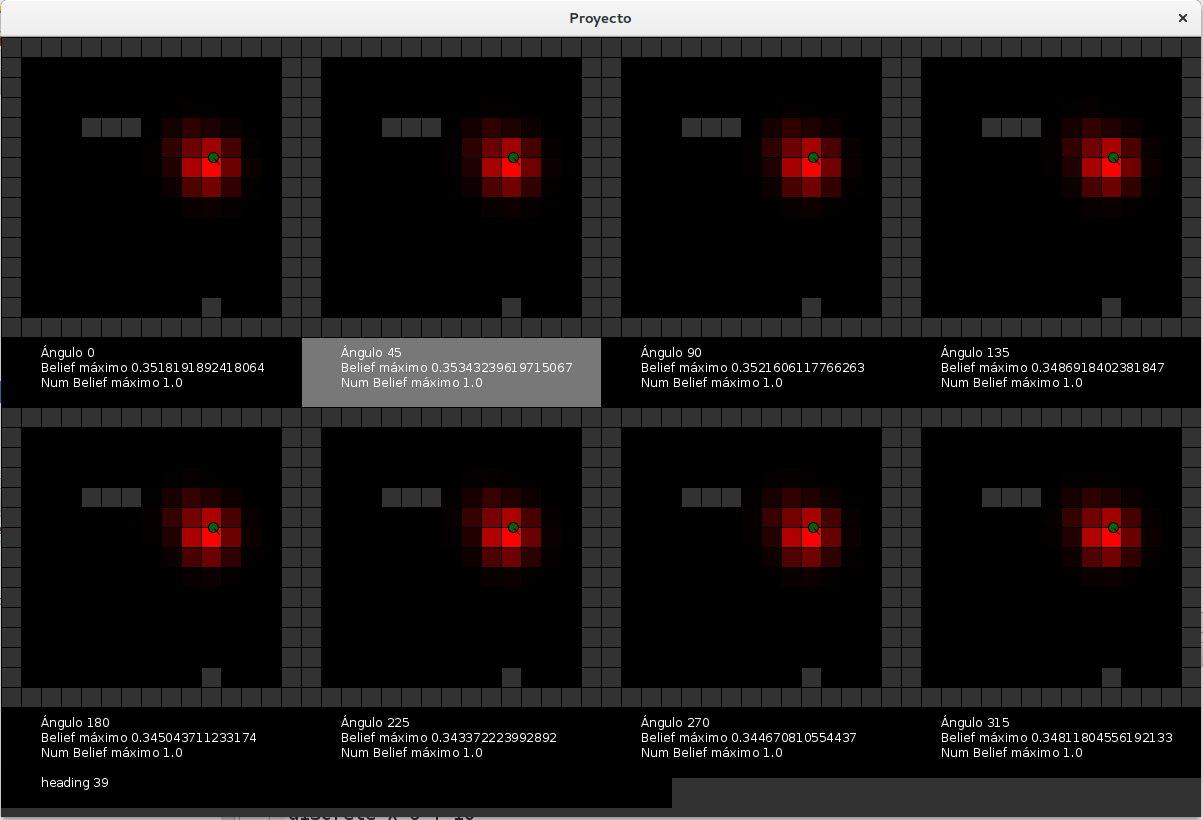
\includegraphics[scale=0.35]{localizacion/mapa_8_dirs.png}
  \caption{Representación del mundo en la mente del robot.}
  \label{fig:mapa2}
\end{figure}

Como habíamos mencionado antes, se necesitará una función que permita obtener la celda en donde se encuentra el robot dadas las coordenadas de éste, pero también se requerirá otra función que nos diga en qué dirección discretizada se encuentra viendo el robot. La función anterior deberá calcular el ángulo al que se encuentra viendo el robot, pero centrado sobre las posibles direcciones de movimiento. Por ejemplo: si el robot se encuentra con una dirección de 12\degree, la función deberá regresar el valor 0\degree, ya que 12\degree \ se encuentra entre (24.5\degree, -24.5\degree].\par

\paragraph{Inicialización}

Deberán posicionar al robot aleatoriamente en el mundo, después deberán calcular la probabilidad de que el robot se encuentre en alguna celda, llamémosle a esta probabilidad \textit{creencia} y representa lo que el robot \textit{cree} acerca de su posición en el mundo \parencite{Dieter1999}. Al inicio esta probabilidad será igual para toda posición porque el robot no sabe dónde está:

\[ P(posici\acute{o}n) = {1 \over \# \ de\ posiciones\ que\ no\ son\ obst\acute{a}culo}\]\medskip

Después, deberán calcular la distancia desde el centro de cada celda al obstáculo más cercano en línea recta, para cada ángulo discretizado. Esta información la deberán guardar para cada posición de tal manera que eviten estar haciendo cálculos cada que sea considerada en el algoritmo siguiente.\footnote{Se sugiere guardar esta información como un atributo de la celda}

\subsection{Notaci\'on}

Definamos la posición discretizada del robot usando una variable tridimensional $l = <x,y,\theta>$, donde $x$ y $y$ son las coordenadas del centro de la celda donde se encuentra el robot y $\theta$ es la dirección discretizada en la que está viendo el robot. A partir de este momento consideraremos únicamente variables discretizadas. Sea $l_t$ la posición real del robot en el tiempo $t$, y $L_t$ la variable aleatoria que modela la probabilidad de que el robot se encuentre en una posición $l$ dada.

Como el robot no sabe su posición exacta, su \textit{creencia} o $Bel(L_t)$ es una distribución de probabilidad \(P(L)\) sobre el espacio de posibles posiciones. Esta \textit{creencia} nos permite saber cuál es la probabilidad de que se encuentre en una celda $l$ en el tiempo $t$, formalmente $Bel(L_t = l)$. Sea \(n\) el número de posiciones posibles.


También aprovecharé para definir a las lecturas de los sensores como: $s_T$ la lectura del láser, $\theta_T$ la lectura del giro y $a_T$ la lectura del sensor odométrico. Sean:

\begin{description}
  \item[$P(s_T \mid l)$] es la probabilidad de que se haya obtenido una medición \(s_T\) si el robot se encuentra en la posición \(l\). Calcularemos esta probabilidad como:
  \begin{align}
    P(s_T \mid l) = {1 \over (\sqrt{2\pi}\sigma_{l\acute{a}ser2})}*\me^{({{-(s_T - \mu_{l\acute{a}ser2})^2} \over {2\sigma_{l\acute{a}ser2}^2}})}
    \label{eq:Pmedicion}
  \end{align}
  donde \(\sigma_{l\acute{a}ser2}\) modela, en parte, el error del sensor y el error por la discretización del mundo, y \(\mu_{l\acute{a}ser2}\) es la distancia desde el centroide de la celda de la posición \(l\) hacia el primer obstáculo.
  \item[$P(\theta \mid \theta', \theta_T)$] es la probabilidad de que el robot esté mirando en el ángulo \(\theta\) de la posición \(l\) dado que se encontraba mirando en el ángulo \(\theta'\) de la posición \(l'\) y se giró un ángulo \(\theta_T\). Supondremos que al girar, el robot no cambia de celda. Calcularemos esta probabilidad como:
  \begin{align}
    P(\theta \mid \theta', \theta_T) = {1 \over (\sqrt{2\pi}\sigma_\theta)}*\me^{({{[\theta_T - (\theta - \theta')]^2} \over {{(\sigma_\theta)}^2}})}
    \label{eq:Podometro}
  \end{align}
  donde \(\sigma_{\theta}\) modela, en parte, el error del sensor y el error por la discretización del mundo. Esta variable será definida por ustedes.
  \item[$P(l \mid l', a_T)$] es la probabilidad de que el robot esté en la posición \(l\) dado que se encontraba en la posición \(l'\) y se avanzó \(a_T\) cms. Calcularemos esta probabilidad como:
  \begin{align}
    P(l \mid l', a_T) = {1 \over (\sqrt{2\pi}\sigma)}*\me^{ -{{1} \over {2}} {{[{ {{ (x' + a_T \cos \theta' - x)^2 } +  { (y' + a_T \sen \theta' - y)^2 } } } + {(\theta' - \theta)^2}]}\over{\sigma^2}}}
    \label{eq:Pgiro}
  \end{align}
  con $\sigma$  modelando el error del sensor.\footnote{Recuerden utilizar radianes, ya que las funciones de \classname{Java} están definidas en radianes.}

\end{description}


Una vez definida la notación, procederemos a ver el algoritmo completo de esta técnica de localización.

 % A estas lecturas se les tendrá que agregar ruido, esto lo lograrán especificando algunas variables:\\

% \begin{enumerate}
%   \item $\sigma$: la varianza de la distribución normal utilizada más adelante.\\
%   \item $S$: porcentaje de ruido de la lectura del odómetro, se usa para calcular $\sigma_x$ y $\sigma_y$.
%   \item $\sigma_\theta$: ruido para la lectura del sensor de giro.
% \end{enumerate}



\subsection{Algoritmo}

\noindent El algoritmo es el siguiente:\medskip

\begin{algorithmic}
  \ForAll{$posicion$ $l$ en $mundo$} \Comment{Inicialización}
    \State $Bel(L_0 = l)\gets P(L_0 = l) = {1 \over n}$
  \EndFor
  \ForAll{$posicion$ $l$ en $mundo$}
    \State $determinar\ las\ distancias\ hacia\ obst\acute{a}culos$
  \EndFor
  \While{$true$}
    \Comment{Se recibió comando o medición del láser}
    \If{no se movió el robot} \Comment{Se recibió medición del láser}
      \State $\alpha_T \gets 0$ \Comment{Constante de normalización}
      \ForAll{$posicion$ $l$ en $mundo$}
        \State $Bel(L_T = l) \gets P(s_T \mid l)*Bel(L_{T-1} = l)$
        \State $\alpha_T \gets \alpha_T + Bel(L_T = l)$
      \EndFor
      \ForAll{$posicion$ $l$ en $mundo$}
      \Comment{Ahora se normaliza la creencia}
        \State $Bel(L_T = l) \gets {\alpha_T}^{-1} * Bel(L_T = l)$
      \EndFor
    \EndIf
    \If{se movió el robot}
      \If{se obtuvo $\theta_T$}
        \Comment{Se obtuvo una lectura del sensor de giro}
        \ForAll{$posicion$ $l$ en $mundo$}
          \State $Bel(L_T = l) \gets [\sum_{\theta'} P(\theta \mid \theta', \theta_T)*Bel(L_{T-1} = l)]$
        \EndFor
      \EndIf
      \If{se obtuvo $a_T$}
        \Comment{Se obtuvo una lectura del sensor odométrico}
        \ForAll{$posicion$ $l$ en $mundo$}
          \State $Bel(L_T = l) \gets [\sum_{l'} P(l \mid l', a_T)*Bel(L_{T-1} = l')]$
        \EndFor
      \EndIf
    \EndIf
  \EndWhile
\end{algorithmic}

\parencite{Dieter1999}

% Si se recibe una lectura del sensor odométrico, por cada celda del mundo, deberán hacer un recorrido por las demás celdas, calculando $\int P(l \mid l', \alpha_T)*Bel(L_T-1 = l')dl$, donde $P(l \mid l', \alpha_T)$ es una variable aleatoria gaussiana tridimensional $G_{x,y,\theta}$ integrada sobre las posiciones de $l$ y $l'$ y desde $\theta + 45\degree/2$ a $\theta - 45\degree/2$.

\subsection{Desarrollo e implementaci\'on}

\subsubsection{Tips}

\begin{itemize}
  \item Tengan bien identificado cuál es su eje X, Y y \(\theta\) en las matrices utilizadas para la simulación.
  \item Utilicen coordenadas polares para todo cálculo, y sólo utilicen grados para visualización, esto les permitirá tener un mayor grado de exactitud y evitan gastar en convertir grados a coordenadas polares en cada operación.
  \item Presten mucha atención en las fórmulas utilizadas, ya que algunas piden sumar la probabilidad sobre un eje, otras piden sumar sobre todas las posiciones del mundo.
  \item Normalicen la creencia cuando el robot gire o se mueva, no solo cuando se reciba una medición del láser. Esto les permitirá compensar errores de redondeo al hacer los cálculos correspondientes.
  \item Hagan una copia del mundo antes de realizar cualquier cálculo, ya que requieren tener la creencia para cada posición en el tiempo \(t-1\) para calcular \(t\). O guarden las creencias recién calculadas en una matriz auxiliar, para luego copiarlas al mundo.
\end{itemize}


\subsection{Requisitos y resultados}

Esto se implementará en processing, recuerden que debe estar bien hecho y comentado, ya que esta práctica vale el 20\% de su calificación. Su aplicación deberá mostrar el mundo, los obstáculos y la probabilidad de cada celda para cada ángulo usando distintos colores o gradientes de un mismo color.

Todo lo anterior lo deberán anexar a la carpeta de la práctica, listo para cargarlo y probarlo. En el \classname{readme} deben especificar cómo se ejecuta, cómo se cargan los archivos, etc. Tampoco olviden comentar su código.




%%
\part{Apéndices}

\appendix
\chapter{Código de prácticas}

\section[Clasificador Bayesiano Ingenuo y Factores]{Clasificador Bayesiano Ingenuo y aplicación de la clase Factor}
\label{appe:aplicaciones}
\subsection{feed.py}
\label{appe:auxiliar}

\begin{minted}[mathescape,
               linenos,
               numbersep=5pt,
               gobble=2,
               frame=lines,
               fontsize=\scriptsize,
               framesep=2mm]{python}
    # -*- coding: utf-8 -*-

    import feedparser
    import urllib3
    import re

    url = 'http://aristeguinoticias.com/feed/'
    db = './feed.db'

    feed = feedparser.parse(url)
    not_in_db = True

    def cleanhtml(raw_html):
        """
        Removes any strange symbol from a HTML string
        """
        cleanr = re.compile('<.*?>')
        cleantext = re.sub(cleanr, '', raw_html)
        return cleantext

    def cleanstr(raw_str):
        """
        Removes any strange symbol from a string
        """
        cleanr = re.compile('&.*?;')
        cleantext = re.sub(cleanr, '', raw_str)
        return cleantext


    for post in feed.entries:
        title = post.title
        link = post.link

        with open(db) as database:
            for line in database:
                if title in line:
                    # Verifying in the entry already exists in the database
                    print('Already in DB')
                    not_in_db = False
                    break

        if not not_in_db:
            not_in_db = True
            continue

        try:
            # Fetching the news data
            http = urllib3.PoolManager()
            r = http.request('GET', post.link)
            data = str(r.data, 'utf-8')
            text = data.split('<div class="class_text">')[1]
            text = text.split('</div>')[0]
            text = cleanhtml(text)
        except Exception as e:
            continue

        summary = cleanstr(text.strip()).replace('\n', ' ')
        tags = map(lambda x: x.term,post.tags)
        tags_clean = ''

        for tag in tags:
            if tag != 'LO + DESTACADO':
                tags_clean = tags_clean + tag + ', '

        tags_clean = tags_clean[:len(tags_clean)-2]

        print("Title: " + title)
        print("Tags: " + tags_clean)
        print("Text: " + summary)
        print("Link: " + link)
        print('')

        with open(db, 'a') as file:
            file.write("Title: " + title + '\n')
            file.write("Tags: " + tags_clean + '\n')
            file.write("Text: " + summary + '\n')
            file.write("Link: " + link + '\n\n')

\end{minted}

\subsection{feed.db}
\label{appe:base}

Si se necesita este archivo, favor de mandar un correo a \href{mailto:luis.lzrg@gmail.com}{luis.lzrg@gmail.com}, ya que por ser un archivo muy extenso decidí no agregarlo.

\newpage

\section[Lego Mindstorms]{Lego Mindstorms}
\label{appe:lego}
\begin{minted}[mathescape,
               linenos,
               numbersep=5pt,
               gobble=2,
               frame=lines,
               fontsize=\scriptsize,
               framesep=2mm]{python}
  from ev3.ev3dev import Motor
  from ev3.lego import ColorSensor

  a = Motor(port=Motor.PORT.A) # Abre el motor en el puerto A
  b = Motor(port=Motor.PORT.D) # Abre el motor en el puerto D
  sense = ColorSensor() # Abre el sensor para leer los valores
                        # que obtiene

  def move():
      maxSpeed = 100
      black = 10
      white = 78
      speedA = 50
      speedB = 50
      midpoint = (white-black)/2 + black
      tolerance = 20
      last_error = 0

      while True:
          # Obtiene el valor de reflectividad de la superficie
          # que ve el sensor
          val = sense.reflect 
          error = midpoint - val
          print error, val

          if abs(error) < tolerance:
              speedA = maxSpeed - last_error/2
              speedB = maxSpeed - last_error/2
              last_error = error
          else:
              if error > 0:
                  speedB = speedB + error/2
                  speedA = speedA - error/2
                  last_error = error
              else:
                  error = abs(error)
                  speedB = speedB - error/2
                  speedA = speedA + error/2
                  last_error = error

          if speedA < 0: speedA = 0
          if speedA > maxSpeed: speedA = maxSpeed
          if speedB < 0: speedB = 0
          if speedB > maxSpeed: speedB = maxSpeed

          # Hace que el motor A gire a la velocidad especificada
          # indefinidamente
          a.run_forever(speedA) 
          # Hace que el motor B gire a la velocidad especificada
          # indefinidamente
          b.run_forever(speedB) 
\end{minted}



%----------------------------------------------------------------------------------------
% Bibliografia
%----------------------------------------------------------------------------------------
\backmatter

\printbibliography[heading=bibintoc]

\end{document}
